\chapter{Numerical Platform}
\label{cha:num}
An essential scientific goal of the GeomInt project is the analysis of potentials and limitations of different numerical approaches for the modelling of discontinuities in the rocks under consideration in order to improve the understanding of methods and their synergies with regard to theoretical and numerical fundamentals. As numerical methods, the continuum approaches "Extended Finite Element Method" (XFEM) and "Phase-Field Method" (PFM), the non-continuous discontinuum methods "Discrete Element Method" (DEM) and "Smoothed Particle Hydrodynamics" (SPH) as well as the hybrid method "Lattice Element Method" (LEM) will be systematically investigated and appropriately extended based on experimental results (Fig. \ref{fig:num-overview}).
\begin{figure}[ht!]
\centering
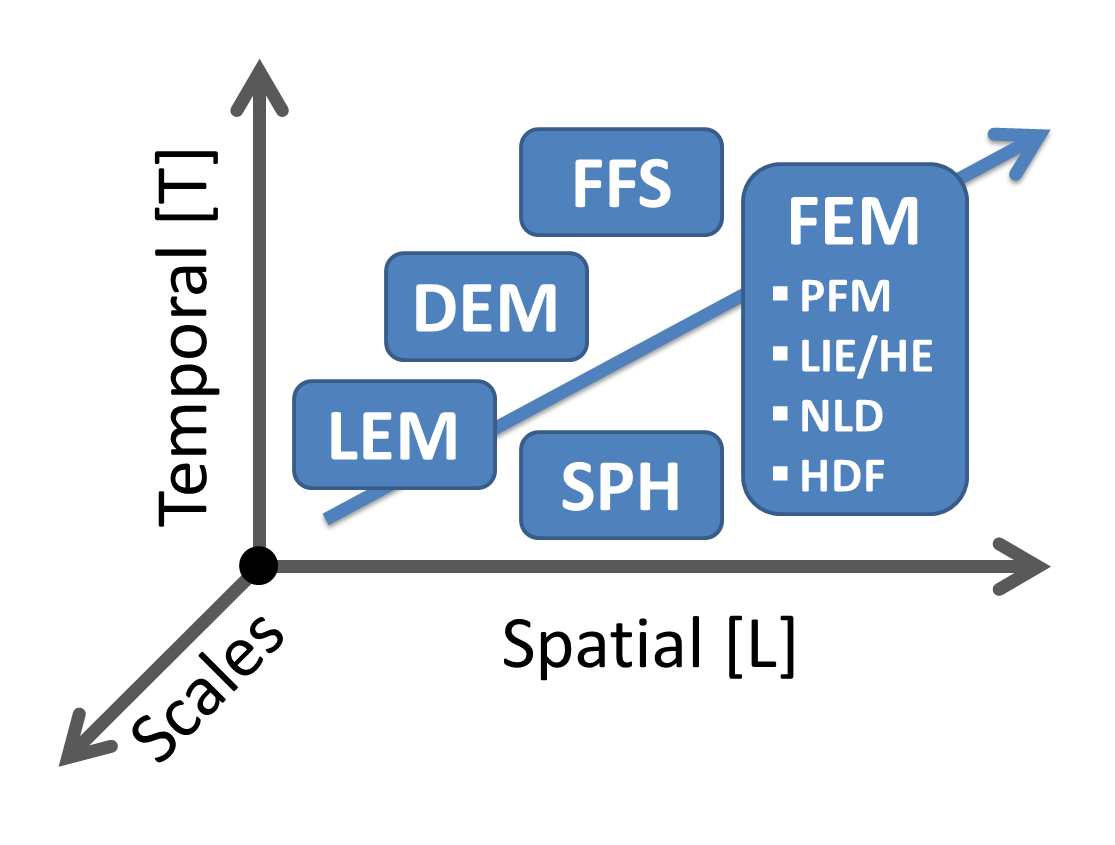
\includegraphics[width=1\textwidth]{figures/geomint-mod-overview}
\caption{Overview of the GeomInt Numerical Platform}
\label{fig:num-overview}
\end{figure}
%--------------------------
\section{State-of-the-Art} 

\subsection{THM simulations and open source development}

Process-oriented numerical simulation programmes are necessary for predicting possible environmental impacts as well as for the macroeconomic and safety design of geosystems for underground use with, if necessary, different or even multiple management. These programmes must be able to represent the running processes and their interactions. Already in the mid-eighties of the last century, specific models were developed in the USA and partly implemented in scientific simulation platforms in order to describe THM processes taking place in the geological subsoil which are connected with the thermal use of the subsoil as energy source (geothermics) or energy storage. However, these investigations primarily had a basic character. In addition, the numerical calculation tools are often oriented towards the description of special processes and only partially consider couplings of different physical processes. Geotechnical applications can also be simulated with a number of established commercial program systems. For hydraulic processes such as multiphase flow in porous media are simulators from the oil and gas industry available (e.g. ECLIPSE, STARS), for the description of mechanical processes as well (FLAC3D). All mentioned codes can only cover a part of the necessary process spectrum. Therefore, simulation programs are required which can represent thermal, hydraulic, mechanical, and chemical (THMC) processes coupled, such as TOUGH \cite{Pruess2004738}, HYTEC \cite{vanderLee2002599}, DuMuX \cite{Flemisch20111102} or OpenGeoSys \cite{Kolditz2012613}. In order to be able to represent the foreseeable impact area of underground use in realistic simulation areas, efforts have been made to parallelise these codes (e.g. OpenGeoSys \cite{Wang20152269}, TOUGH \cite{Wu2002243}). In particular, the simulation of systems subject to discontinuity requires high performance computing. A major limitation of commercially available numerical simulation programs is that their source codes are not accessible and therefore not transparent and that a further development of such programs is therefore only possible by the commercial developer. In the research project applied for here, the platforms OpenGeoSys (UFZ (coordinating), BGR, CAU, IfG, TUBAF), mD-LEM (CAU) and pythonSPH (Uni Stuttgart) developed by some of the applicants as open source software can be used, so that the limitations mentioned do not exist. The description of discontinuities with different approaches described in the following as well as their processing in the sense of high-performance computing (HPC) requires targeted program extensions.
\index{HPC High-Performance-Computing}

\subsection{Continuum models (XFEM and variational phase field)}

In recent years, extended \cite{Belytschko1999601} or also known as generalized \cite{Strouboulis200043}  finite element methods (XFEM/GFEM) and phase-field methods \cite{Bourdin2000797} for the description of existing and developing discontinuities and singularities within continuum mechanical approaches have established themselves ahead of all others. 
Both methods differ fundamentally and have their own strengths and weaknesses. 
XFEM locally extends the approach and test function space by formulations that can map the discontinuous course of the solution and introduces corresponding additional local degrees of freedom. 
Usually, this approach is combined with so-called level set methods, which help to localize the discontinuity and thus ultimately determine in which elements the solution space has to be extended. 
This approach allows the approximation of discontinuous solutions on comparatively coarse grids, but requires programmatic infra-structures for the treatment of flexible additional degrees of freedom, level sets and other aspects, which require a considerable implementation effort, especially in branched crack systems. 
In contrast, the variational phase field method was originally proposed as a generalized Griffith criterion by~\cite{Francfort1998} and numerically implemented using a phase-field variable by~\cite{Bourdin2000}.
In the variational phase-field model, cracks are represented by a smoothly varying function (phase-field variable) that transitions from intact material (phase-field variable = 1.0) to fully broken state (phase-field variable = 0.0) using a regularization parameter with the dimension of a length and the energy consumed by the cracks is computed from this diffused representation. 
One of the strengths of this approach is to account for arbitrary numbers of pre-existing or propagating cracks in terms of energy minimization, without any a priori assumption on their geometry or restriction on the growth to specific grid directions.

XFEM \cite{Belytschko1999601} was originally developed for crack propagation problems and was also applied in the geotechnical context, e.g. for multiphase flows \cite{Chessa200310},\cite{Mohammadnejad2013327} and heat transport \cite{Khoei2012701},\cite{Shao2014155}. Current developments of generalized and extended finite element methods in the context of hydraulic stimulation are mainly concerned with the efficient coupling of solid-state and flow-mechanical problems \cite{Yazid20094269},\cite{Watanabe20121010},\cite{Meschke2015438}.

The variational phase-field model of fracture has witnessed wide ranging applicability in from dynamic fracture~\cite{Bourdin2011},\cite{Borden2012},\cite{Li2016}, to ductile fracture~\cite{Ambati2015},\cite{Miehe2015486}, \cite{Alessi2017}, to thermal and drying fracture~\cite{Maurini2013},\cite{Bourdin2014},\cite{Miehe2015_thermo}. 
The first application of the variational phase-field model to hydraulically driven crack propagation has been proposed by~\cite{Bourdin2012} and followed by many others~\cite{Wheeler2014},\cite{Wilson2016},\cite{Heider201738},\cite{Santillan2017},
\cite{Chukwudozie2019957},
\cite{Li201942} 
or for land slide modeling \cite{Wei2020} 
with various formulation and numerical implementation. 
While the reported findings are promising thus far, the method still needs more establishments for practical field scale applications. 
The required efforts may include validation against laboratory/field experiments, approaches to recover explicit properties such as fluid leak-off from smeared crack representation, and more complex physics phenomena such as visco-elasticity.
\index{VPF Variational Phase Field method}

\subsection{Discontinuum models}

Discontinuum models directly map forces of interaction between predefined discrete elements. The latter may themselves be discretized and mapped by continuum mechanics. Decisive for the mapping of developing discontinuities, however, are the pre-defined interfaces subject to certain interface formulations. This type of modelling was applied in geotechnics, for example, to geothermal systems \cite{Zeeb2015264} and has also made a decisive contribution to the simulation of the pressure-driven generation of flow paths in polycrystalline salt rocks, which is bound to the discontinuum-mechanical microstructure of the salt rocks. Polycrystalline salt rocks represent a discontinuum of intergrown salt crystals on the micromechanical level. In contrast to porous media, there is no cross-linked pore space in salt rocks. Only by pressure-driven opening and cross-linking of pathways, i.e. generation of connectivity by opening channels along the grain boundaries of the salt crystals, cross-linked flow paths are created in salt rocks. Fluid pressure-driven percolation is direction-dependent and seeks the path of least resistance along the crystal grain boundaries in the polycrystalline salt rock under the effect of the existing stress field. This mechanism of directional percolation can be simulated in coupled HM models on a discontinuity mechanical basis.

The observations on numerical models of pathogenesis by source and shrinkage processes based on a microscale based analysis must be able to map significant structural changes and discontinuity developments in nonisothermal HM coupled processes, which manifest themselves in progressive fracture or self-healing processes under pressure, saturation and temperature influence. First basics of the modelling of fracture processes on the microscale were published at the end of the 1990s with reference to self-organising fracture processes based on Voronoi discretizations \cite{BolanderJr.1998569}. By combining the approaches of HM modelling in saturated media \cite{Asahina201413} and TM modelling \cite{Rizvietal2016}, the connection for the simulation of self-organizing fracture processes in geomaterials shall be established with consideration of complex TH$^2$M processes. Based on the elasticity theory, linear fracture models following Mode I and Mode II were developed for fragile, largely homogeneous material with few inclusions. For materials with high interference, models based on continuum fracture mechanics \cite{Talreja1991165} were developed which require specific information on material microstructure and fracture behaviour. Thermal conductivity in cemented geomaterials is determined by heat transfer between mineral particles, porosity, fluid and contact quality 
\cite{Woodside19611688},\cite{Bahrami20063691},\cite{Widenfeld200315}.
The Thermal Particle Dynamics method can be used to simulate the transient heat propagation in granular media and the associated thermal expansion \cite{Vargas20011052}. This was considered in a thermal DEM \cite{Vargas20023119},\cite{Vargas2007}, but the calculation effort is enormous and the grain or contact shape is greatly simplified \cite{Zhang2011172}. In contrast to the particle methods, the heat propagation in cemented materials can be determined numerically very effectively by classical FEM, but microlevel information disappears due to the underlying homogenization. This poses a problem for the initiation of discontinuities by thermal processes in THM coupling. 

The hybrid lattice models have been developed to tackle the shortages in continuum based models, such as the simplicity to define the heterogeneity/anisotropy as well as the fracture simulation and stress redistribution during the frack propagation (discontinuities) without the need to re-mesh the domain \cite{Bolanderetal1998, vanMieretal2002}. The lattice model is similar to the finite volume (FVM) or finite difference (FDM) methods, with the difference that the FVM or FDM explicitly discretize the continuum \cite{Rizvietal2018a, Rizvietal2018c}. The simplicity and accuracy of lattice models to simulate the fracking in cemented geomaterials, such as rock and concrete \cite{Liuetal2007, Pradoetal2003, Karihalooetal2003}, are well established. The lattice models in comparison to the continuum methods are time consuming and expensive. Therefore, their applicability and development in real engineering applications or commercial softwares are not well developed. However, with the increase of computational power during past years as well as the implementation of parallel computing or GPU computing methods, the application of lattice models in commercial softwares is imminent.
\index{LEM Lattice Element Method}

The mentioned DEM approaches, as classical discontinuum models, have the disadvantage that additional connections between the particles have to be implemented by beam elements, which contain the fracture-mechanical criteria. Lattice based models - LEM \cite{Chessa200310, Chung199615094} have been developed for modeling of fracture mechanical processes considering discontinuity and crack initiation as well as crack propagation. These include a networking of the existing heterogeneity ranges (Voronoi and Delaunay triangulation) and use simple linear fracture criteria on the microscale. The cross-linked two- and three-dimensional continuum regions are microscopically coupled by 1D elements in the center of gravity of the Voronoi cells. In the simplest case these elements are Hookesche springs with a normal stiffness \cite{Curtin1990535}. In three-dimensional space these simple springs already give a good approximation of the Mode I failure model \cite{Wong2015417}. With the use of Born spring models and an additional tangential degree of freedom, shear behaviour can already be modelled \cite{Jagota19933123}. By extending the spring, for example as a beam element \cite{Schlangen1992435}, displacements, rotations and moments can be transferred to the node in addition to the forces, whereby an additional bending contact can be taken into account \cite{Sahimi1993713}. For the spatial lattice network thus generated, the displacements at each point are determined by generating an equilibrium or by minimizing the energy \cite{Meakin1991226} or dynamic relaxation \cite{Cundall197947}. The LEM combines the advantages of simple implementation with the ability to control particle interaction in the model while simultaneously self-organizing initiation and progression organization of a discontinuity, \cite{Sattarietal2019b, Wuttke201785}.
\index{DEM Discrete Element Method}

Additionally, in contrast to discrete models, the lattice models can be implemented to represent a continuum, as the lattice elements do not necessarily define the particle to particle contact mechanics \cite{Rizvietal2019a}. The hybrid lattice model can represent a continuum or particle-to-particle contacts, depending on the objective of the simulation. In both cases, the domain is discretized into series of spring or beam elements, representing the bonds. The regularization of a lattice model grants the independency of the results from the mesh size and meshing technique \cite{Ostojastarzewski2002}. The lattice models were initially emerged in order to simulate the fracture initiation and propagation in cemented geomaterials. With the time, lattice models have been extended to simulate the wide variety of the thermal \cite{Shresthaetal2019, Rizvietal2019d, Rizvietal2016}, thermo-mechanical \cite{Sattarietal2017, Sattarietal2019b} and hydro-mechanical \cite{Grassl2009} problems in the engineering applications. In the recent years, the hybrid lattice models have been extended to determine the granular, cemented or swelling geomaterials response under the coupled thermo-hydro-mechanical (THM) processes.

\subsection{Smoothed Particle Hydrodynamics}
\index{SPH Smoothed Particle Hydrodynamics}

Smoothed Particle Hyrodynamics (SPH) methods are reticule numerical collocation methods for solving partial differential equations. SPH methods were formulated almost 40 years ago to solve astrophysical problems and have been further developed in recent years to solve a variety of problems and models in fluid and solid state mechanics \cite{Monaghan2011323}. The SPH method is particularly suitable for problems with free surfaces or material interfaces such as discontinuities and cracks: SPH methods are Updated or Total Lagrange methods, i.e. boundary conditions at discontinuities can be described numerically well. In recent years, great progress has been made in the efficiency of SPH formulations, especially for questions with internal interfaces, such as for non-Darcy flows in porous media or in the multiphase fluidics of immiscible fluids in porous media \cite{Morris2000333},\cite{Tartakovsky2005610}. The so-called "Whole Domain Formulation", i.e. a numerical procedure in which the surface conservation equations (mass and momentum), such as the Young-Laplace equation in multiphase fluidics, are "smeared" by means of the kernel function and integrated into the bulk conservation equations (Continuum Surface Force - CSF), can be interpreted here as a "phase field method" which "continuously smears" the physical properties of the discontinuities. Besides the consideration of the SPH-inherent kernel function in the CSF methods and the absence of the need to artificially adduce discontinuities, the net-free SPH methods above all show great efficiency advantages when complex and small-scale (pore) geometries are to be precisely mapped \cite{Sivanesapillai2016212}. In addition to small-scale direct numerical simulations on the pore space scale, SPH methods for coupled HM problems in geomechanics have already been developed \cite{Bui2007339},\cite{Bui20141321}. The two HM-coupled biotubes poroelastic equation sets for the porous solid phase and the viscous pore fluid were formulated in these works with two disjunctive particle sets which can lead to difficulties in impulse interaction modelling. A further development of the SPH method for HM processes, also taking into account propagating discontinuities such as cracks and crack networks, is therefore imperative to establish the SPH method as an efficient and reliable tool for geoscientific problems.

All the approaches described above have proved to be suitable in principle for the physical analysis of the growth of discontinuities. However, in connection with the extension of the methods to coupled THM processes, there is still a fundamental need for development in many areas. This is to be supported by an improved process understanding to be worked out, by building on it some of the numerical methods used here are to be further developed purposefully beyond the state of the art. Applications that go beyond the simulation of laboratory experiments and use the methods for solving practically motivated problems of large-scale geosystems have so far hardly been found in the literature or have not even been developed for certain essential process couplings. There is an urgent need for systematic investigations into the questions of how these methods can be translated into practical applications, what computing resources are required, and in which cases certain methods appear more suitable than others. The aim of this project is to develop such an overall view and a systematic comparison of the methods at defined benchmarks as well as their embedding in proven software, partly with the inclusion of methods of high performance computing.
%--------------------------
\section{Numerical Methods}
%--------------------------
\subsection{FFS - Forces on Fracture Surfaces}
\label{chap:NumPlatf:FFS}
\begin{figure}[htb!]
\begin{center}
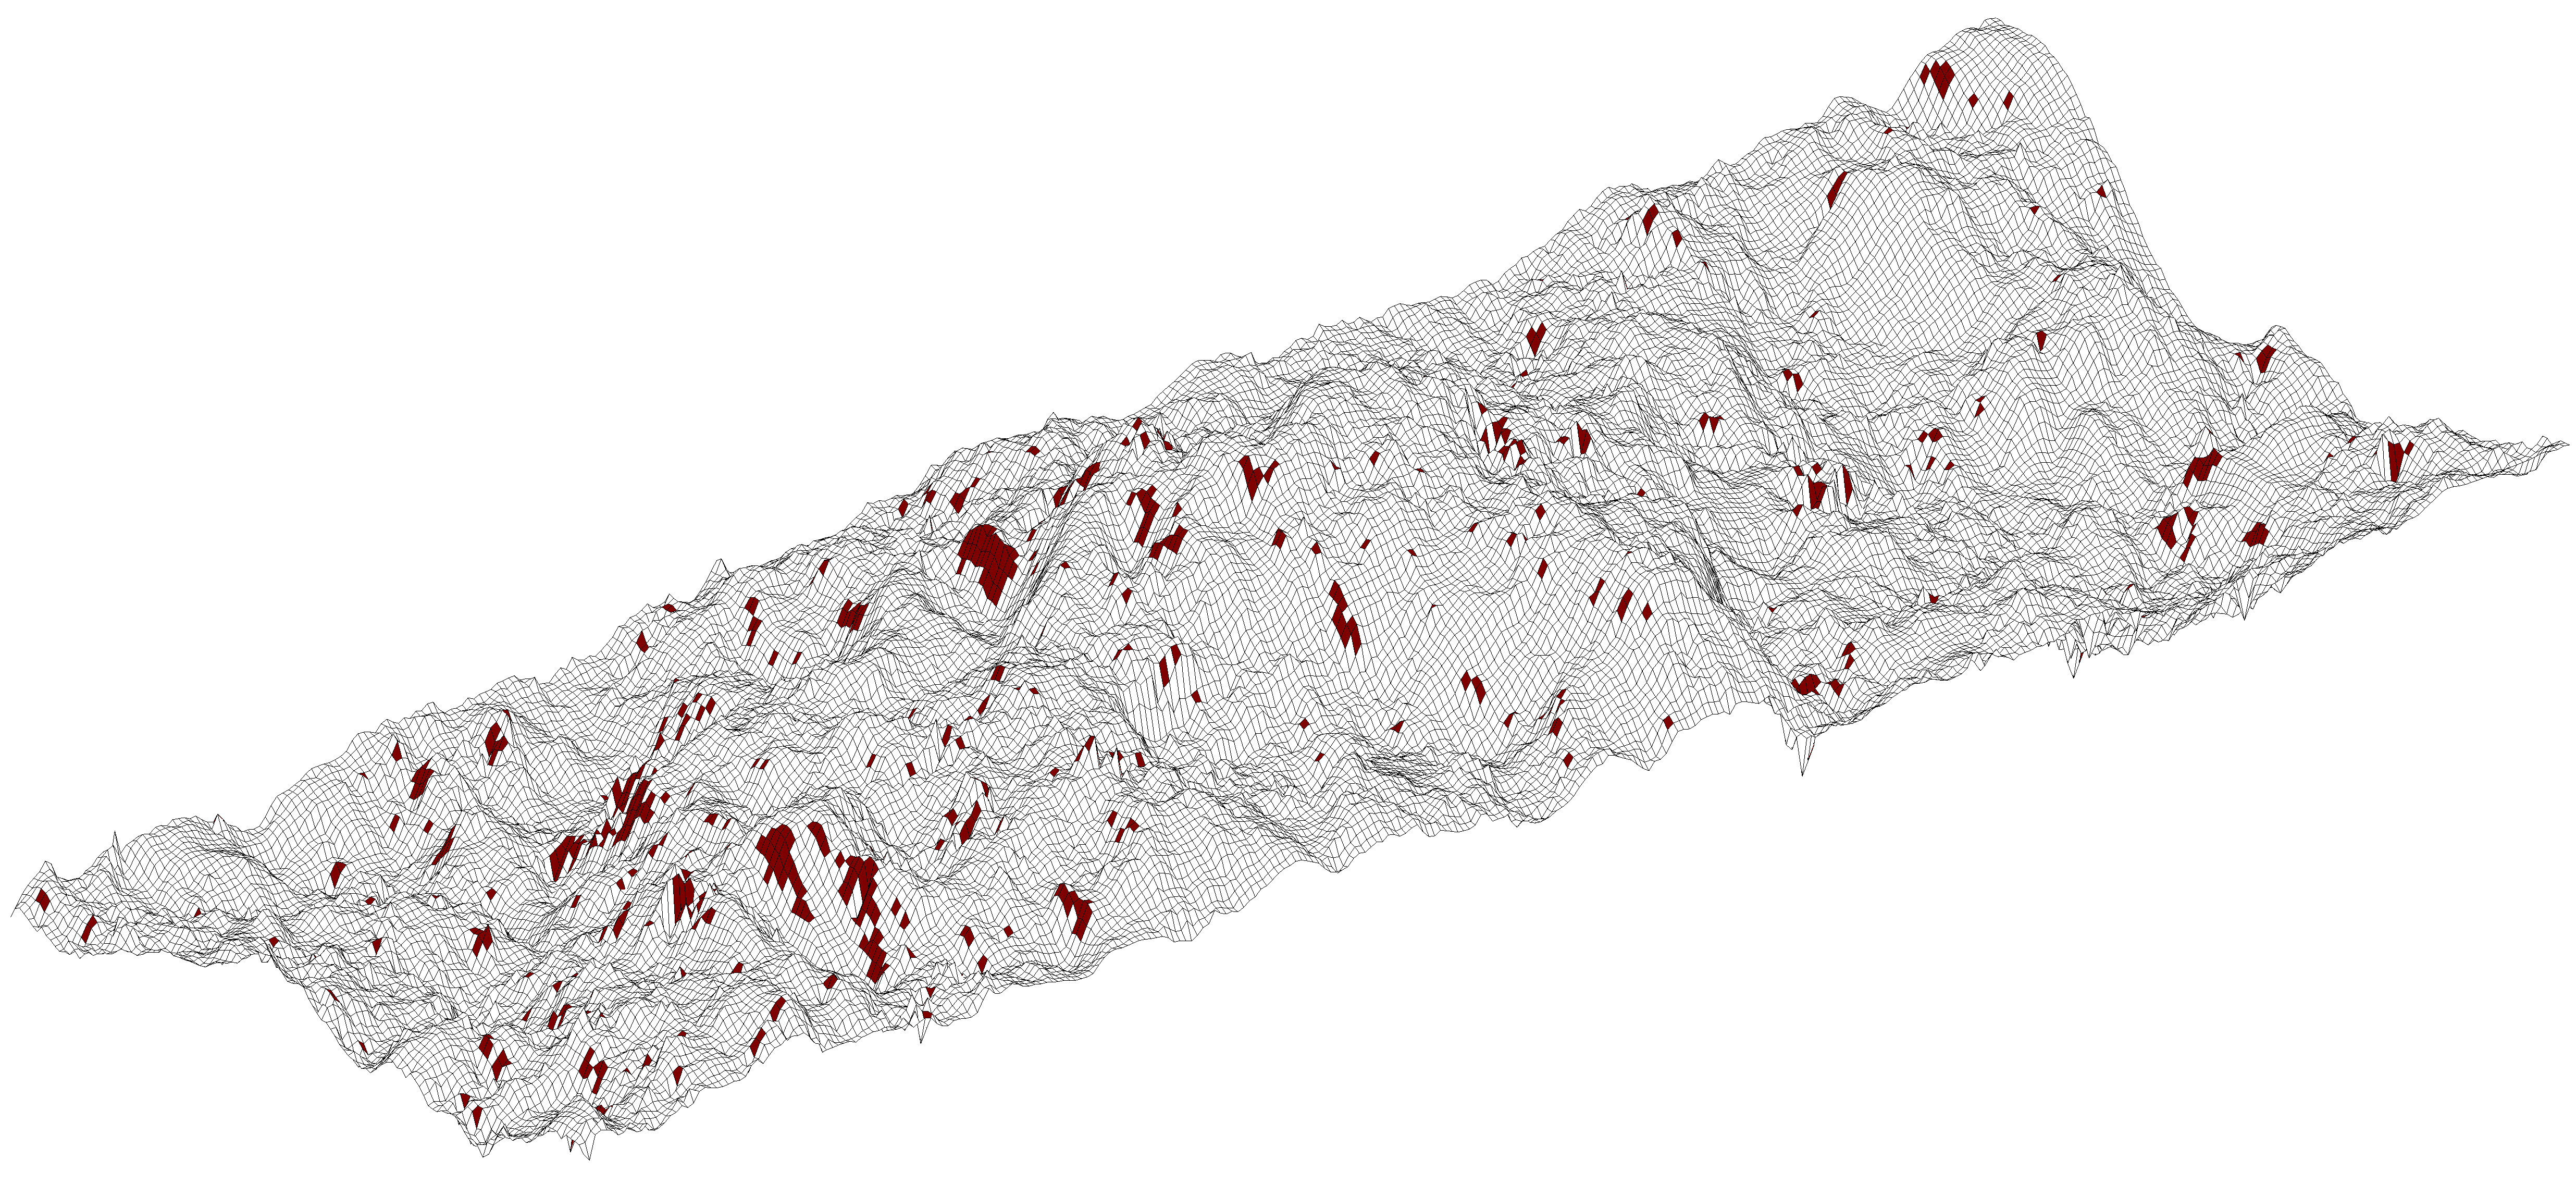
\includegraphics[width=0.6\textwidth]{./figures/FFS_MarkedSurfaceElements.png}
\end{center}
\caption{The elements used in a shear test simulation are marked in red. The FFS approach is able to look directly inside a model and helps to deepen the understanding of the active processes.}
\label{Fig:FFS-MarkedElements}
\end{figure}
This numerical method explicitly uses the geometry of a rock surface and calculations on single surface elements are executed. The main advantage of this method is the possibility to closely look inside the mechanisms which control the shear behaviour of the joint (Figure \ref{Fig:FFS-MarkedElements}). The drawback is the high computation time needed due to the more complex calculation scheme.\\
Starting point were the works by \cite{Fathi2016} and \cite{Casagrande2017}. The last mentioned work uses a FFS approach. The geometry of surface is represented as a triangular surface. The apparent dip angles $\theta^\ast$ for the elements are calculated. An iterative scheme decides whether the surface can slide over its counterpart or whether the surface elements in contact are destroyed. In the case of destruction the geometry is corrected and the next check for sliding versus destruction starts. The two important formulas are the one for the sliding forces: 
\begin{equation}
F_{slide}=F_{loc} \cdot \tan (\varphi_b + \theta^\ast)
\end{equation}
where $F_{loc}$ is the local force acting on one element, $\Phi_b$ is the basic friction and $\theta^\ast$ the apparent dip angle of this element.\\
The other formula is the one for shear forces, which is the force needed to destroy the surface element:
\begin{equation}\label{eq:shear}
F_{shear}=A \cdot (c + \sigma_{loc}*tan(\Phi))
\end{equation}
where $A$ is the ground area of the element, $c$ the cohesion of the rock material, $\sigma_{loc}$ the local normal stress and $\Phi$ the angle of inner friction of the rock material.



\begin{figure}[htb!]
\begin{center}
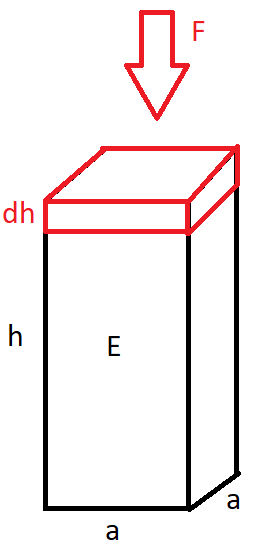
\includegraphics[width=0.2\textwidth]{./figures/FFS_NormalForce.png}
\end{center}
\caption{A surface element is represented as a rock column which with\-stands normal forces by elastic deformation.}
\label{Fig:FFS-NormalForce}
\end{figure}
The idea of the newly developed approach is to have a physically consistent calculation scheme. Therefore the normal forces of the surface elements in contact have to be estimated. The simplest approach was chosen to keep things manageable. An elastic stress-displacement behaviour was basically used (Figure \ref{Fig:FFS-NormalForce}). The resulting formula is:
\begin{equation}
F_n= \sum_i E * a^2 * \frac{\Delta h_i}{h}
\end{equation}
For all $i$ surface elements in contact the relative height change $\frac{\Delta h}{h_i}$, the ground area $a^2$ and the Young's modulus $E$ were used. For a specific rock joint the two surfaces are moved towards each other until the force created by the elastic deformation equals the force which is applied to the fracture.\\
\ \\
Another simplification compared to \cite{Casagrande2017} is the usage of quadratic grid elements. This allows to store the height values in a matrix form which is easy to handle.  
%--------------------------
\subsection{LEM - Lattice-Element-Method}

The application of the lattice element in modeling the fracture initiation and propagation in the geomaterials is well established \cite{Liuetal2007, Pradoetal2003, Vanmieretal2002}. The main advantage of the LEM over other numerical methods is the ability to model the stress redistribution and concentration upon the fracking process. The application of the LEM is extended to model the heat transfer in cemented geomaterials \cite{Sattarietal2017} as well as non-cohesive granular particles \cite{Rizvietal2018b}. The thermo-mechanical lattice model based on the integration of the interface element is able to model the expansion and shrinkage processes during the heating and cooling cycles \cite{Sattarietal2019b}. The LEM is also implemented to model the foam concrete behavior under the dynamic loading \cite{Rizvietal2018a}. In the recent decade, the dual lattice model to simulate the coupled hydro-mechanical loadings in geomaterials is developed \cite{Grassl2009}. In these models, the dual mesh grid for the fluid transport is generated. The short description of the implemented coupled thermo-hydro-mechanical lattice method is given below.

\subsubsection*{Discretization of the domain}

The domain is discretized into a series of Voronoi cells to represent the individual particles or a continuum depending on the purpose of the investigation. With the application of the vectorized random lattice (VRL), the irregularity factor known as the randomness factor ($\alpha_{R}$), which varies between 0 and 1, is introduced \cite{Moukarzeletal1992}. When the randomness factor is 0, the generated mesh is regular and when it is equal to 1, it reaches the maximum irregularity for VRL model.  Afterward, the Voronoi Tessellation is implemented and polygonal cells are generated (see Figure \ref{fig:Amir_LEM_Domain_2D}, \ref{fig:Amir_LEM_Domain_3D}). The Delaunay Triangulation process results in the Voronoi cell connectivities, which are defined as the bond elements between two adjacent nodes. 

\begin{figure}[!ht]
\begin{subfigure}[c]{0.48\textwidth}
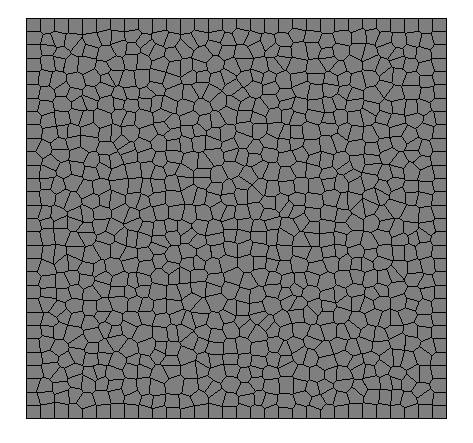
\includegraphics[width=1\textwidth]{figures/Amir_LEM_Domain_2D.png}
\subcaption{}
\label{fig:Amir_LEM_Domain_2D}
\end{subfigure}
\hfill
\begin{subfigure}[c]{0.48\textwidth}
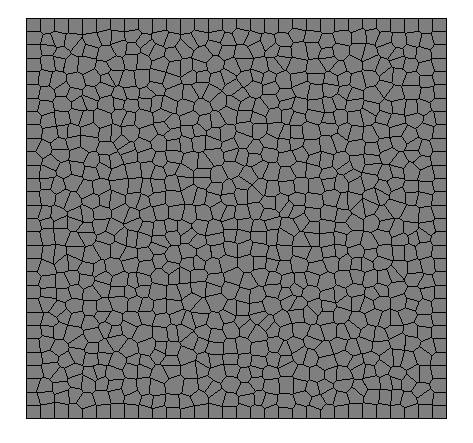
\includegraphics[width=1\textwidth]{figures/Amir_LEM_Domain_3D.png}
\subcaption{}
\label{fig:Amir_LEM_Domain_3D}
\end{subfigure}
\caption{The generated domain with $\alpha_{R} = 0.5$ (a) 2D discretization, and (b) 3D discretization}
\end{figure}

\subsubsection*{Mechanical lattice model}

The mechanical lattice model is based on the assumption of the Mode I and II linear elastic fracture mechanics. The simulation of the fracture in LEM is based on the removal of the bond elements between the neighboring Voronoi cells \cite{Rizvietal2019a}. The elements strength threshold is defined based on the critical strain energy or the fracture toughness for Mode I and II. In a different approach, the strength threshold is defined based on the Mohr-Coulombs tension cutoff model \cite{Bolanderetal1998}. The lattice elements are represented by series of spring (1DOF),  Euler-Bernoulli beam (3DOF)(Figure \ref{fig:Amir_LEM_Beam}) or Timoshenko beam elements (4DOF). The regularization of the regular lattice model, such as a triangular or square discretization technique, is carried out and a relationship between the continuum and element properties is presented \cite{Ostojastarzewski2002, Karihalooetal2003}. This regularization assumes that the stored strain energy of a continuum, $U_{\mathbb{R}}$, is equal to the stored strain energies in each individual Voronoi cells, $U_{Cell}$. The strain energy stored in a unit cell depends on the total number of each cells bond elements ($N_b$), the elements response forces ($F_b$) and the response displacements ($u_b$). For a continuum, the stored energy depends on the continuum stresses ($\sigma_{\mathbb{R}}$) and continuum strains ($\varepsilon_{\mathbb{R}}$) throughout the continuum volume ($V_{\mathbb{R}}$).

\begin{figure}[!ht]
\centering
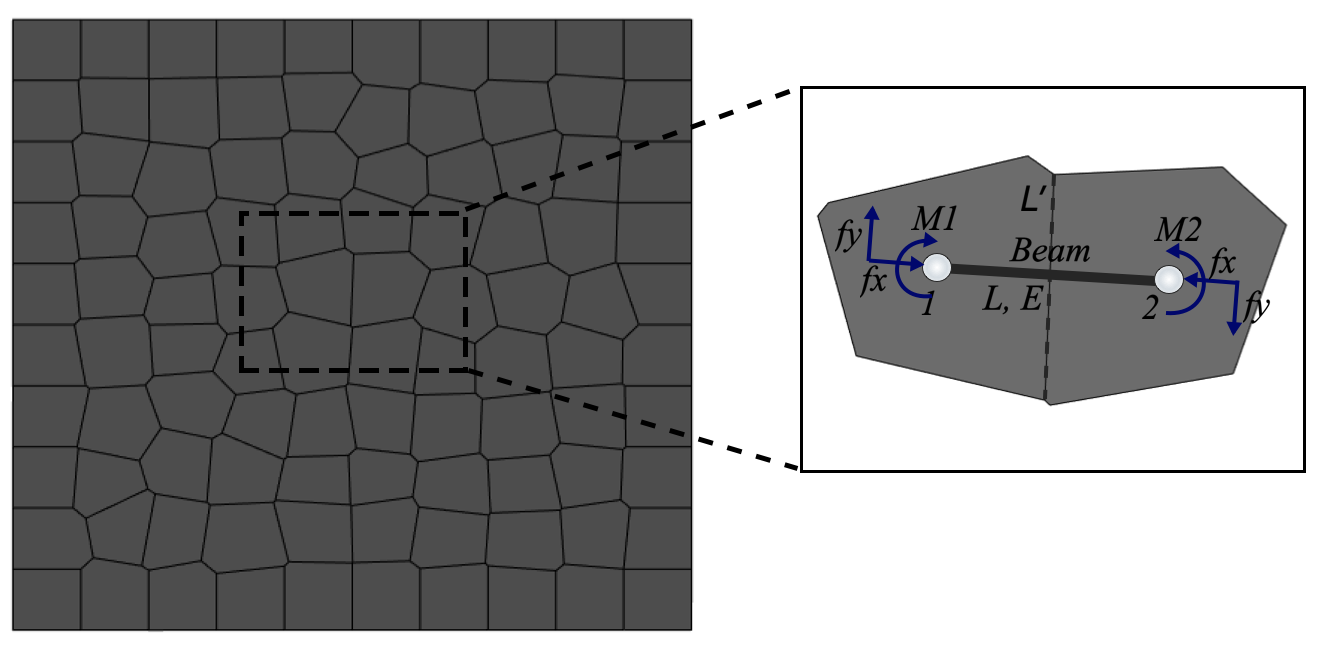
\includegraphics[width=0.75\textwidth]{figures/Amir_LEM_Beam.png}
\caption{The Euler-Bernoulli beam element representing the bond between two cells}
\label{fig:Amir_LEM_Beam}
\end{figure}

\begin{equation}
\label{eq:LEM_Mechanical_1}
 U_{Cell}=U_{\mathbb{R}}
\end{equation}

\begin{equation}
\label{eq:LEM_Mechanical_2}
 U_{Cell}=\frac{1}{2}\sum_{b=1}^{b=N_b}F_b.u_b
\end{equation}

\begin{equation}
\label{eq:LEM_Mechanical_3}
 U_{\mathbb{R}}=\frac{1}{2}\int_{V_{\mathbb{R}}}{\sigma_{\mathbb{R}}.\varepsilon_{\mathbb{R}}.dV}
\end{equation}

For a discretized 2D domain with the spring element, the length of the element ($L_b$), alignment orientation ($n_{i,j,k,m}$), first stiffness coefficient ($(R)^\prime$), continuum stiffness matrix $C_{\mathbb{R}}$, and strains of $\varepsilon_{i,j,k,m}$ are correlated as,

\begin{equation}
\label{eq:LEM_Mechanical_4}
U_{Cell}=\frac{1}{2}\sum_{b=1}^{b=N_b}L_b^2.((R)^\prime.n_i.n_j.n_k.n_m.\varepsilon_{ij}.\varepsilon_{km})_b
\end{equation}

\begin{equation}
\label{eq:LEM_Mechanical_5}
U_{\mathbb{R}}=\frac{1}{2}\varepsilon_{\mathbb{R}}.C_{\mathbb{R}}.\varepsilon_{\mathbb{R}}
\end{equation}

For a Euler-Bernoulli beam element in 2D, the curvature strain ($\kappa_{i,j}$), curvature stiffness ($D_{i,j}$), stiffens matrix ($C_{i,j,k,m}$) and second stiffness coefficient ($(R)^{\prime\prime}$) are related as,

\begin{equation}
\label{eq:LEM_Mechanical_6}
U_{\mathbb{R}}=\frac{V}{2}\varepsilon_{ij}C_{ijkm}\varepsilon_{km}+\frac{V}{2}\kappa_{i}D_{ij}\kappa_j
\end{equation}

\begin{equation}
\label{eq:LEM_Mechanical_7}
C_{ijkm}=\sum_{b=1}^{b=N_b} ({n_i.n_k \left( n_j.n_m.(R)^\prime)+n_j.n_m.(R)^{\prime\prime} \right)})_b
\end{equation}


After the regularization of the lattice model and with the minimization of the potential energy of the system, the load Vs. displacement relation in each time step is determined. For a single element, the stored total strain energy ($U_t^b$) is equal to the sum of axial ($U_a^b$), shear ($U_s^b$) and moment ($U_m^b$) strain energies. Eventually, the total strain energy depends on the axial force ($f_x$), shear force ($f_y$) and moment ($M_b$) along the element's length of $z=0:L_b$, the area of elements ($A_b$), element's shear modulus ($G_b$), element's Young's modulus ($E_b$), and moment of inertia ($I_b$). The bi-linear softening scheme is implemented to model the quasi-brittle material behavior existing in rock and concrete geomaterials \cite{Inceetal2003}. The measured $E_b$ values depends on the peak strain ($\varepsilon_p$), failure  strain ($\varepsilon_f$), current element strain ($\varepsilon_b$) and peak load ($f_p$) where the stiffness degradation starts.

\begin{equation}
\label{eq:LEM_Mechanical_8}
 U_t^b(z)=U_a^b(z)+U_s^b(z)+U_m^b(z)=\frac{1}{2}\int_{0}^{L_b}{\left(\frac{f_x{(z)}^2}{E_b A_b}+\frac{f_y{(z)}^2}{G_b A_b}+\frac{M_b{(z)}^2}{E_b I_b}\right).dz} 
\end{equation}

\begin{equation}
\label{eq:LEM_Mechanical_9}
E_b=\frac{f_p}{\varepsilon_f-\varepsilon_p}\left(\frac{\varepsilon_f}{\varepsilon_b}-1\right)
\end{equation}

\subsubsection*{Thermo-mechanical lattice model}

The thermo-mechanical lattice model is based on the weak coupling scheme between the thermal and mechanical models, which decreases the computational costs. The thermal lattice model is based on the discrete thermal lattice model (TDEM) \cite{Zhangetal2011, Fengetal2008}, where the Hertzian contact model is implemented to account for the heat conductance ($h_b$) between the particles. The axial compression force increment ($f_x$) results in higher thermal conductance between the particles, which eventually leads in a higher effective thermal conductivity ($K_{eff}$). The regularization of the thermal lattice model is based on the relationship between the heat conductivity of elements and the continuum \cite{Rizvietal2018b}. The $h_b$ depends on the contact length ($L_b^\prime$) (or area in 3D domain), contact forces and assigned elements thermal conductivities ($k_{b}$).

\begin{equation}
\label{eq:LEM_Thermal_1}
h_b = k_{b} \left( (L_b^\prime)+ \left(\frac{3f_x L_b}{4E_b}\right)^\frac{1}{3} \right)
\end{equation}

In a steady state, the amount of the heat in- and outflow ($q_b$) from a Voronoi cell (Figure\ref{fig:Amir_LEM_Thermal}) is equal to zero,

\begin{figure}[!ht]
\centering
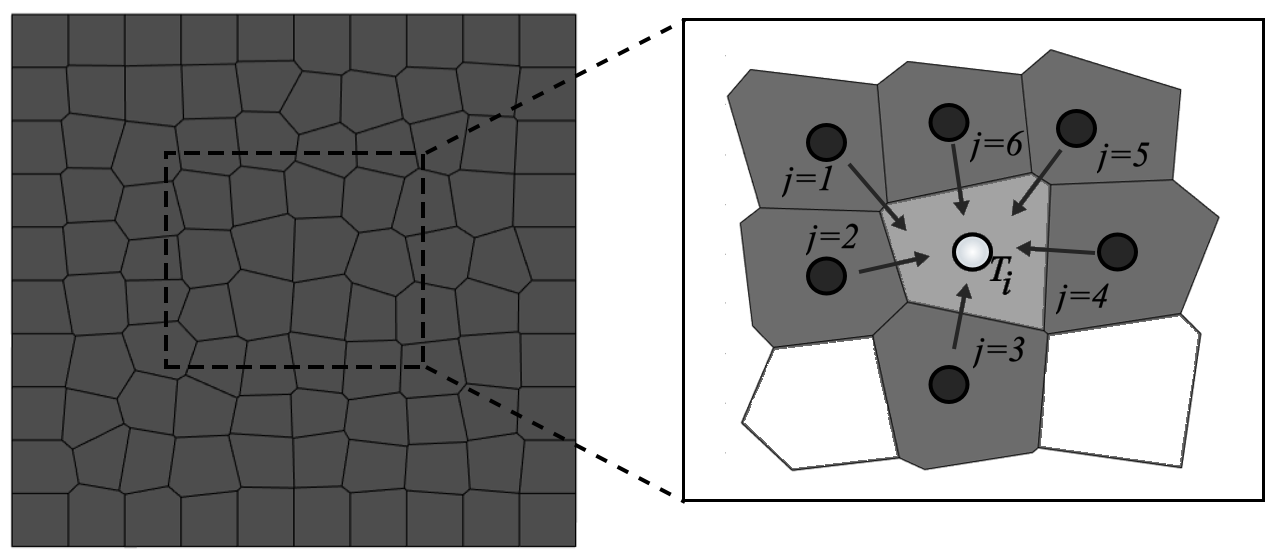
\includegraphics[width=0.75\textwidth]{figures/Amir_LEM_Thermal.png}
\caption{The heat flow into $i_{th}$ cell from surrounding boundaries}
\label{fig:Amir_LEM_Thermal}
\end{figure}


\begin{equation}
\label{eq:LEM_Thermal_2}
\rho_{i}c_{i}v_{i}\frac{dT_{i}}{dt}-\nabla .\left(k_i\nabla T_i\right)-\rho_i{\dot{q}}_i=0
\end{equation}

\begin{equation}
\label{eq:LEM_Thermal_3}
\nabla .\left(k\nabla T_i\right)=\sum_{b=1}^{b=N_b}{q_b}=\sum_{b=1}^{b=N_b}{h_b(T_i - T_j)_b=0}
\end{equation}

 
where, $\dot{q}$ is heat density (assumption: $\dot{q}=0$), $t$ is time, $\rho_{i}$ is density, $c_{i}$ is heat capacity and $v_{i}$ is the volume of each Voronoi cell ($i$). In a transient case,

\begin{equation}
\label{eq:LEM_Thermal_4}
\sum_{b=1}^{b=N_b}{q_b=}\rho_{i}c_{i}v_{i}\frac{dT_i}{dt}
\end{equation}

The effective thermal conductivity is calculated based on the average volume technique, where $q_{ave}$ is the average heat flow, $q_{Cell}^{b}$ is the heat flow through the assigned cells located in the boundary ($N_C$), $\dot{T}$ is the temperature gradient and  $\hat{x}_{cell}$ is the relative coordinates of each cell.

\begin{equation}
\label{eq:LEM_Thermal_5}
q_{ave}=\frac{\sum_{b=1}^{b=N_C}q_{Cell}^b.\hat{x}_{Cell}}{V}
\end{equation}

\begin{equation}
\label{eq:LEM_Thermal_6}
q_{ave}=K_{eff}.\dot{T}
\end{equation}

The thermal strain is calculated based on the linear expansion of the lattice elements and the given heat expansion coefficient. The implementation of the thermal expansion into the mechanical model results in a fully coupled thermo-mechanical model \cite{Sattarietal2019b}.

\subsubsection*{Hydro-mechanical lattice model} \label{Section:HMLattice}

The existing hydro-mechanical lattice models are based on the assumption of the dual lattice network, where the mechanical lattice elements transfer the mechanical loads between the two nodes and the conduct elements perpendicular to the alignment of the mechanical elements transfer the fluid or gas flow between the conduct nodes \cite{Grassl2009, Grassletal2013}. The implemented hydro-mechanical lattice model is based on the mass conservation ($m_f$) of the fluids in the continuum. The hydraulic aperture ($a_h$), fluid density ($\rho_f$),  fluid viscosity ($\nu_f$), flow length ($L_b^\prime$), hydraulic resistance ($R_h$), saturation degree ($Sr$) and bulk modulus ($K_f$) are the main parameters used to determine the hydraulic pressures ($P_f$) and transferred fluid masses ($\Delta m_f$) between the conduct nodes. 

\begin{equation}
\label{eq:LEM_Hydro_1}
m_f^{t+1}=m_f^t+\Delta m_f
\end{equation}

\begin{equation}
\label{eq:LEM_Hydro_2}
m_f^{t=0}={\rm Sr}^{t=0}V_{cav}\rho_f\left(1+\frac{P_f^{t=0}}{K_f}\right)
\end{equation}

\begin{equation}
\label{eq:LEM_Hydro_3}
\Delta m_{f,ij}=f\left(Sr\right).\frac{P_{f,j}-P_{f,i}-\rho_fg\left(Z_j-Z_i\right)}{R_h}.\Delta t
\end{equation}

where, $Z$ is the relative coordinate of the $i,j$ conduct nodes, $V_{cav}$ is the volume of the cavity, $g$ is the gravity and $f(Sr)$ is the saturation function which is equal to 0 and 1 in a dry and saturated conditions, respectively. According to the finite-discrete element method (FDEM) \cite{Lisjaketal2017}, the fluid mass is stored within defined physical and artificial cavities. Each conduct node represents an artificial cavity connected through conductive elements (Figure \ref{fig:Amir_LEM_Hydro}), where the hydraulic conductivity is governed based on the parallel plate cubic flow rule. 

\begin{figure}[!ht]
\centering
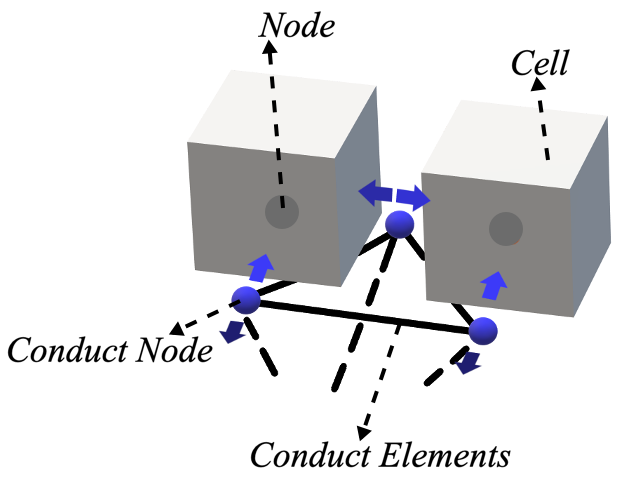
\includegraphics[width=0.75\textwidth]{figures/Amir_LEM_Hydro.png}
\caption{The schematic representation of the implemented hydro-mechanical model}
\label{fig:Amir_LEM_Hydro}
\end{figure}

\begin{equation}
\label{eq:LEM_Hydro_4}
R_h = \frac{12\nu_f}{a_h^3} L_b^\prime = 12 \nu_f \int_{z_i}^{z_j} \frac{1}{a_h (z^3)}dz= \frac{6 \nu_f (a_{h,j}+a_{h,i})}{(a_{h,i} a_{h,j})^2} L_b^\prime
\end{equation}


When an artificial cavity is saturated, the amount of excessive fluid mass flowing inside the cavity builds the pore pressure, which then is transmitted into the mechanical nodes. If the cavity is not saturated, then the pore pressure is assumed to be zero. 

\begin{equation}
\label{eq:LEM_Hydro_5}
P_f^t=P_f^{t-1}+K_f\frac{\Delta m_f}{\rho_fV_{cav}^t}\ \ \ \ \ \ \ \ \ \ \ if\ \ \ \ {\rm Sr}^t=1
\end{equation}


With the implementation of the pore pressures into the mechanical lattice nodes, the pore pressure diffusion and the change of the hydraulic conductivity with the crack opening and closure are measured. The flow simulation is implemented under both the pressure- and flowrate controlled boundary conditions.


\subsubsection*{Shrinkage and swelling lattice model} 

The simulation of the shrinkage and swelling using the lattice element method is based on the particle shrinkage model \cite{Simaetal2013}, which is mainly considered in the discrete models. In contrast to the DEM, the shrinkage in LEM is implemented into the lattice elements (Figure \ref{fig:Amir_LEM_Shrinkage}). To do so, the interface elements to represent the bond between the particles are generated (\cite{Sattarietal2019b}). The shrinkage and swelling coefficients ($\alpha_s$) are temperature dependent. According to the initial water content ($\omega^{t=0}$) and the change of the water content during the shrinkage and swelling process, the linear strain in the lattice elements is determined and implemented into the mechanical model. 

\begin{figure}[!ht]
\centering
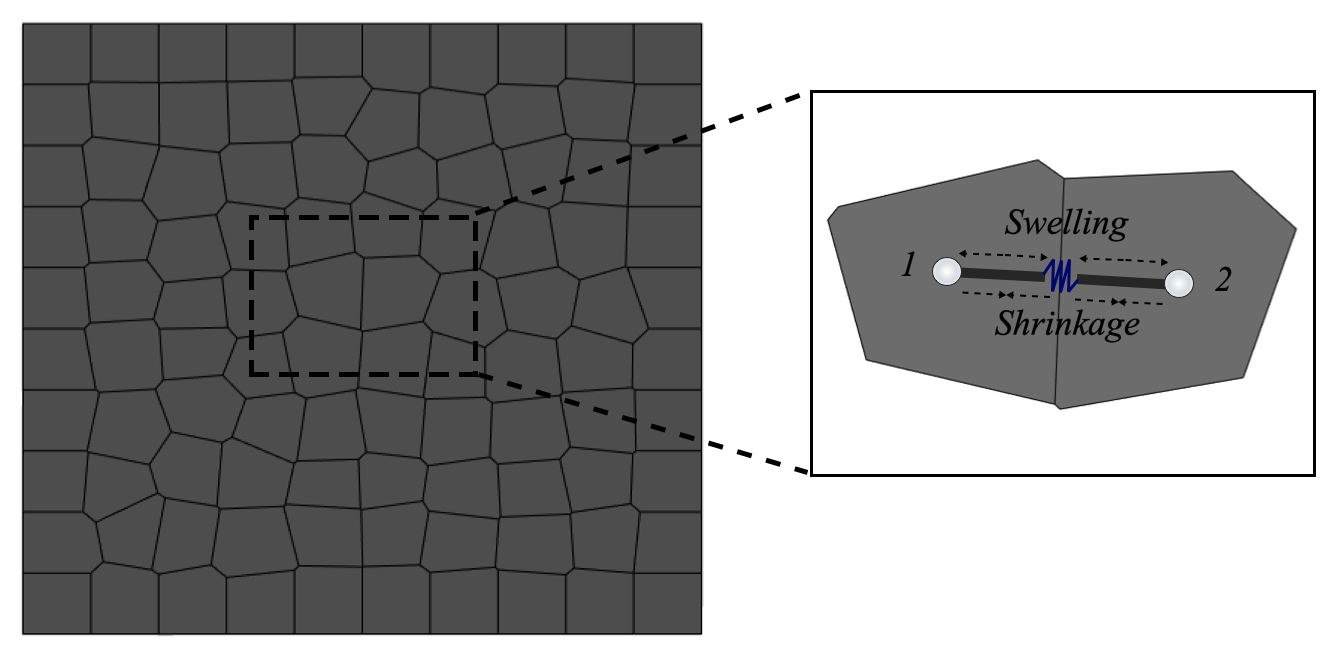
\includegraphics[width=0.75\textwidth]{figures/Amir_LEM_Shrinkage.png}
\caption{The implementation of the interface element to simulate the shrinkage and swelling processes}
\label{fig:Amir_LEM_Shrinkage}
\end{figure}

\begin{equation}
\label{eq:LEM_Shrinkage_1}
L_b^t=L_b^{t=0}e^{-\alpha_s.\frac{t}{t=\infty}}
\end{equation}

\begin{equation}
\label{eq:LEM_Shrinkage_2}
\alpha_s=-\frac{1}{3}\ln{(1-\frac{\omega^{t=0}-\omega^{t}}{1+e_0}}.G_s)
\end{equation}


The shrinkage and swelling coefficient are time, temperature and depth dependent. Therefore, graphs representing the evaporation rate as well as the soil water characteristic curves to assess the applied suction and the water content during the wetting and drying paths are required \cite{Voetal2017}. $\bar{\bar{\sigma}}$ and $\bar{\bar{\varepsilon}}$ are the stress and strain tensors, respectively. 

\begin{equation}
\label{eq:LEM_Shrinkage_3}
\bar{\bar{\sigma}}=C:\bar{\bar{\varepsilon}}-Sr.P_f\bar{\bar{\delta}}
\end{equation}

The elements shrinkage and expansion results in the axial compression and tensile stresses in the lattice elements, which when they exceed their predefined strength threshold are removed and the micro fracking process under shrinkage and swelling conditions is simulated.

%--------------------------
\subsection{DEM - Distinct-Element-Method}
\todo[inline]{IfG: short DEM description}
%--------------------------
\subsection{SPH - Smoothed-Particle-Hydrodynamics}
\index{Smoothed-Particle-Hydrodynamics (SPH)}
Direct Numerical Simulations (DNS) of effective physical properties of single-phase flow through porous or fractured solid materials can be performed directly on the pore scale of the porous soil or rock. Morphological information, the basis for the subsequent DNS, is obtained as segmented (binarized) voxel-data from $\mu$ X-Ray Computed Tomography (XRCT). In general, numerical simulations of flow processes on XRCT-data at small to moderate Reynolds (Re) numbers could be performed by mesh-based Finite Element, Finite Differences or Finite Volume methods.
% \todo{HS: References} %
\index{direct numerical simulation (DNS)}
\index{Reynolds number (Re)}
\index{XRCT}

Here, we haven chosen the mesh-less Smoothed Particle Hydrodynamics methods as an alternative simulation technique. SPH is a Lagrangian simulation tool used to solve Partial Differential Equations (PDE) and was originally developed for astrophysical problems \cite{gingold1977smoothed,lucy1977numerical}. In recent years, due to it's flexibility and
scalability and applicability on HPC architectures, especially in an explicit formulation,
it became attractive for various problems fluid dynamics like single and multi-phase fluid mechanics with internal interfaces, suspension flow, and single and multi-phase flow in porous media  \cite{sivanesapillai2016csf,sivanesapillai2016pore,sivanesapillai2014transition,sivanesapillai2018fluid,markauskas2017comparative}.%\todo{Nadine's work} 
Within the framework of this method, the discretisation of the PDEs spans a set of interacting collocation points $\mathcal{P}_i$ with position vectors $\Tx_i$, referred to as particles. The positions of the particles represent integration points at which field functions $\Phi (\Tx, t) $ are interpolated by convolution with the Dirac-Delta function $\delta$:
\index{Lagrangian methods}
\index{collocation method}
\index{Dirac-Delta function}

\begin{equation}
\label{eq:SPH_dirac_delta}
\Phi (\Tx, t) \, = \, \int_\Omega \Phi (\Tx', t) \delta(\Tx - \Tx') \dv.
\end{equation}

Replacing $\delta(\Tx -  \Tx')$ with the kernel function $ W(\Tx - \Tx', h)$ results in the approximation

\begin{equation}
\label{eq:SPH_replacement_kernel}
\Phi (\Tx, t) \, \approx \, \int_\Omega \Phi (\Tx', t) W(\Tx  -  \Tx', h) \dv,
\end{equation}

where the support $h$ of the kernel determines a sphere of influence and likewise declares neighbouring particles $\mathcal{P}_j$ with position vector $\Tx_j$. Subsequently, the discretisation (numerical integration) of the integral formulation converts continuous field functions into discrete particle properties  $\Phi (\Tx_i) = \Phi_i$, kernel representations into spatial discretisation and equation \glref{eq:SPH_replacement_kernel} yields 

\begin{equation}
\label{eq:SPH_discrete_field_function}
\Phi_i \, = \, \sum_j^N \Phi_j W(\Tx_i  -  \Tx_j, h) V_j \, .
\end{equation}

Herein, $V_j$ is introduced as the discrete representation of $ \dv$ and $j \, = \, 1,2, \dots, N $ indicates the neighbour particles within the kernel support of particle $\mathcal{P}_i$. Analogously, differential operators turn into short-range interaction forces. For more technical details, also accounting to the necessary time integration we refer to \cite{monaghan2012smoothed,sivanesapillai2016pore,ye-2019}.

\subsubsection{Single-phase flow of a Newtonian fluid}
\index{Newtonian fluid}

A SPH implementation of single-phase flow of a Newtonian fluid is based on the solution of the balance of momentum in the present local form

\begin{equation}
\label{eq-40_sph}
\rho^\Gf \,\dot{\Tv}_\Gf \, = \, \mu^\Gf \div (\grad \Tv_\Gf) \, - \, \grad p \, + \, \rho^\Gf\,\Tb \end{equation}
and the balance of mass
\begin{equation}
\label{eq-50_sph}
 \dot{\rho}^\Gf \, = \, -\rho^\Gf \div \Tv_\Gf \, ,
\end{equation}
which are known as the Navier-Stokes equations.
\index{Navier-Stokes equations}
We adopted the notation used in mixture theory 
\cite{steeb-2019b,steeb-2019a}
where a subscript is used for kinematical quantities and a superscript elsewhere.
$\rho^\Gf (\Tx, t)$ is the mass density field, $\Tv_\Gf $ is the velocity vector, $\mu^\Gf $ is the dynamic viscosity, $p (\Tx, t)$ is the pressure field and $\Tb$ are body force densities.
The ``dot'' operator, cf. Equations \glref{eq-40_sph} and \glref{eq-50_sph},
is denoting the material or substantial time derivative $\cdot{(\bullet)} = \partial_t{\bullet} + \grad(\bullet) \cdot \Tv_\Gf$.
In order to solve the quasi-incompressible (weakly compressible) character of the Navier-Stokes equations an equation of state for the pressure in the form
$p(\rho^\Gf)$ has to be formulated.
\index{weakly incompressible SPH}
\index{quasi-incompressible SPH}
Therefore, either a linear model or the Tait equation \cite{hayward1967compressibility}
\index{Tait equation}
\index{equation of state (EoS)}

\begin{equation}
\label{eq:SPH_tait_eos}
p(\rho^\Gf) \, = \, \frac{\rho_0^\Gf\,c^2_\Gf}{\gamma} \Bigg[ \Big( \frac{\rho^\Gf}{\rho_0^\Gf} \Big)^\gamma \, - \, 1 \Bigg]
\end{equation}

is commonly employed, wherein $c_\Gf = \sqrt{K^\GF}{\rho^\Gf}$ is the speed of sound of the fluid with the bulk modulus $K^\Gf$ and $\gamma$ is 
a constant, specific to the modeled problem (usual $\gamma \, = \, 7 $ for quasi-incompressible fluids).
%\todo{HS: Gleichung (6) muessen wir nochmals kurz diskutieren. Was genau is $\rho$ und was wird fuer $\rho_0$ gewaehlt? } 

\subsubsection{Discrete equations}

By applying the above introduced transformation from continuous field equations to discrete algebraic SPH equations, the total force on each fluid particle $\mathcal{P}_i$ is obtained as the sum of the discrete body forces $\TF_i^B =  m_i\,\Tb $, viscous interaction forces $\TF_{ij}^V$ and pressure interaction forces $ \TF_{ij}^P$

\begin{equation}
\label{eq:SPH_momentum_balance}
m_i \dot{\Tv}_i \, = \, \sum_j^N \TF_{ij}^P  + \sum_j^N \TF_{ij}^V + \sum_j^N \TF^B,
\end{equation}
which leads to a relation for the particle velocity update
\begin{align}
\label{eq:SPH_update_velocity}
\dot{\Tv}_i \, = \, & - \, \sum_j^N m_j \Big( \frac{p_i}{{\rho_i}^2} + \frac{p_j}{{\rho_j}^2} \Big) \frac{\Tx_{ij}}{r_{ij}} \frac{\partial W_{ij}}{\partial r_{ij}} \, \\ 
& + \, \sum_j^N \frac{m_j (\mu_i + \mu_j)(\Tv_i - \Tv_j)}{\rho_i \rho_j} \Big( \frac{1}{r_{ij}} \frac{\partial W_{ij}}{\partial r_{ij}} \Big) \, + \, \Tb \, .
\end{align}

Reconfiguration of the balance of mass, cf. equation \glref{eq-50_sph} yields 

\begin{equation}
\label{eq:SPH_discrete_mass_balance}
\dot{\rho}_i \, = \, \sum_j^N m_j (\Tv_i - \Tv_j) \cdot \frac{\Tx_{ij} }{r_{ij}} \frac{\partial W_{ij}}{\partial r_{ij}}.
\end{equation}

However, the density field can also be calculated by an accumulative kernel interpolation $\rho_i = \sum m_j W_{ij}$.
%\todo{HS: Auch hier muessen wir wieder aufpassen. Was fuer ein $\rho$ meinen wir?}

\subsubsection{Boundary conditions, time integration and artificial viscosity}

For the application of single-phase flow though porous media, the solid skeleton is considered to be rigid and fluid-solid interfaces $\Gamma^{FS}$ generally satisfy no-slip and no-penetration boundary conditions. 
More general solid-fluid interaction phenomena could be considered in SPH formulations, e.g. to mimic rough rock surfaces with asperities, but are not further discussed in the following.
%\todo{HS: haetten wir hier auch noch ein Zitat?}
To that end, the solid domain is populated by so-called ``dummy'' particles
\cite{sivanesapillai2016pore,ye-2019}. The velocity and pressure of these dummy particles is extrapolated by the fluid phase and computed by the balance of momentum, respectively, following the method proposed by Adami et al.~\cite{adami2012generalized}. Resulting velocity and pressure fields of dummy particles are counteracting those of the fluid phase and thus create no-slip and no-penetration conditions on $\Gamma^{FS}$. 
The discrete particle properties are updated by the Velocity Verlet time integration method \cite{swope1982computer, verlet1967computer} which is a common time-integration scheme in particle methods. Further, a dissipative artificial viscosity term is used to reduce non-physical oscillations, e.g. \cite{monaghan1992smoothed,ye-2019,monaghan2012smoothed}.  
\index{artificial viscosity}
\todo[inline]{UoS: Are all important symbols listed?}
%--------------------------
\subsection*{FEM - Finite-Element-Method}
In the following we briefly introduce some extensions of the Finite-Element-Method which particularly are suited for fractured-porous media analysis and fracturing processes.
%--------------------------
\subsection{LIE - Lower-Interface-Elements}
%--------------------------
The following implementation is based on \cite{Watanabe2012} and represents a special case of extended finite element methods~\cite{Moees1999,Belytschko2009,belytschko2001arbitrary} in that the enrichment is limited to element boundaries. 
The implementation is here extended to cohesive zone traction separation laws, cf.~\cite{needleman1990analysisa,needleman1990analysisb,nguyen2001cohesive,Elices2002,Gasser2005,Meschke2007}.

\subsubsection*{Weak form}
The weak form of the static equilibrium equation $\mdiv \mbfs{\sigma} + \varrho \mathbf{b} = \mbf{0}$ can be written as the principle of virtual work
\index{static equilibrium equation}
\index{principle of virtual work}

\begin{equation}
\int_{\Omega \setminus \Gamma_\mrm{c}} \delta \bm{\epsilon} \dcdot \bm{\sigma} \, \mathrm{d} \Omega - \int_{\Omega \setminus \Gamma_\mrm{c}} \delta \mbf{u} \cdot \varrho \mbf{b} \, \mathrm{d} \Omega - \int_{\partial_\mrm{N}\Omega} \delta \mathbf{u} \cdot \bar{\mathbf{t}}\, \mathrm{d} \Gamma - \int_{\Gamma_{\mathrm{c}}} \underbrace{\left(\delta \mathbf{u^{+}} - \delta \mathbf{u^{-}}\right)}_{\delta [\![\mathbf{u}]\!]} \cdot \mathbf{t}_{\mathrm{c}} \, \mathrm{d} \Gamma = 0,
\label{eq:weak_form_equil_eq}
\end{equation}

where $\delta \mbf{u}$ is the first variation of the displacement field (virtual displacements), $\mathbf{u^{+}}$ and $\mathbf{u^{-}}$ denote displacements of the opposing fracture phases such that $[\![\mathbf{u}]\!] = \mathbf{u^{+}} - \mathbf{u^{-}}$ is the displacement jump across the interface, $\bar{\mathbf{t}}$ and $\mathbf{t}_{\mathrm{c}}$ are the boundary ($\partial_{\mrm{N}}\Omega$) and the interface ($\Gamma_\mrm{c}$) traction, respectively. While the boundary traction $\bar{\mathbf{t}}$ is given by the applied external forces along the contour, the interface traction $\mathbf{t}_{\mathrm{c}}$ follows from a constitutive response of the interface according to the the relative displacement between the opposing surfaces. Note, that the above definition implies stress continuity between the matrix compartments across the interface, $\mathbf{t}_{\mathrm{c}} = \mbfs{\sigma}(\mbf{x}_\Gamma) \mbf{n}^+_\Gamma = - \mbfs{\sigma}(\mbf{x}_\Gamma) \mbf{n}^-_\Gamma$.

\subsubsection*{Constitutive model}

While the matrix material behaves according to linear elasticity and is assumed to be impermeable in the current study, the crack will be fluid saturated and follows an effective stress-type formulation:
\index{effective stress}
\begin{equation}
\mbf{t}_\mrm{c} = \mbf{t}'_\mrm{c} - p_\mrm{f} \mbf{n}_\Gamma,
\label{eq:effective_LIE}
\end{equation}
where the fluid pressure in the fault only acts on the normal traction across the fault, not its shear components. For the effective stress, a cohesive-zone law has been implemented based on the following assumptions:
\index{cohesive zone model}

\begin{list}{-}{\leftmargin=1em \itemindent=0em \itemsep=0em}
\item Damage is driven by fracture opening $[\![\mathbf{u}]\!]\cdot\mbf{n}_\Gamma$ only, i.e. only mode I fracture propagation is considered.
\item The traction-separation law is bilinear.
\item Cleavage unloading (in contrast to ductile unloading) is considered in view of modelling brittle fracture. 
\end{list}

The cohesive zone model is characterized by its peak tensile normal traction or normal tensile strength $t_\mrm{n,p}$, its initial normal and shear stiffness $K_\mrm{n}$, $K_\mrm{s}$, and its fracture toughness/critical energy release rate $G_\mrm{c}$. 

The undamaged elastic fracture constitutive law 
\begin{equation}
	\mbf{t}'_\mrm{c} = \mbf{K} \jump{\mbf{u}} = \left[ K_\mrm{n} (\mbf{n}_\Gamma \otimes \mbf{n}_\Gamma) + K_\mrm{s} (\mbf{I} - \mbf{n}_\Gamma \otimes \mbf{n}_\Gamma) \right] \jump{\mbf{u}},
\end{equation}
remains valid in compression ($w_\mrm{n} = \jump{\mbf{u}} \cdot \mbf{n}_\Gamma < 0$). During compressive loading, a penalty formulation 
\begin{equation}
	K_\mrm{n}^\mrm{pen} = K_\mrm{n} \left[1 + \ln^2 \left( \frac{b}{b_0}\right) \right],
\end{equation}
based on current ($b$) and initial ($b_0$) aperture is invoked to prevent fracture face interpenetration at high compressive loads. 

In tension, the model is modified to account for damage
\begin{equation}
\mbf{t} = \mbf{K}^\mrm{d} \jump{\mbf{u}}.
\end{equation}
During monotonously increasing loading, damage evolves linearly with normal fault opening between the limiting values
\begin{equation}
	d =
	\begin{cases}
		0  &  w_\mrm{n} = w_\mrm{n,p}\\
		1   &  w_\mrm{n} = w_\mrm{n,f},
	\end{cases}
	\label{eq:coh_param}
\end{equation}
where $ w_\mrm{n,p} = \frac{t_\mrm{n,p}}{K_\mrm{n}}$ and $ w_\mrm{n,f} = 2 \frac{G_\mrm{c}}{t_\mrm{n,p}}$.
%
Damage is implemented as a non-decreasing function according to:
\begin{equation}
	d^{t+\Delta t} = \text{min}\, \left[1, \text{max}\, \left( \frac{\langle w - w_\mrm{n,p} \rangle}{w_\mrm{n,f} - w_\mrm{n,p}}, d^t \right) \right],
	\label{eq:d_LIE}
\end{equation}
where the Macauley brackets have been used.
\index{Macauley brackets}
%
The new tensile normal stiffness is found via
\begin{align}
	K_\mrm{n}^\mrm{d} = \frac{t_\mrm{n}}{w_\mrm{n}} = \frac{(1-d) t_\mrm{n,p}}{\underset{0\leq \tau \leq t}{\text{max\,}}w_\mrm{n}(\tau)} = \frac{(1-d) K_\mrm{n} w_\mrm{n,p}}{d(w_\mrm{n,f} - w_\mrm{n,p})+ w_\mrm{n,p}}.
\end{align}
Accordingly, the entire stiffness tensor is degraded:
\begin{equation}
	\mbf{K}^\mrm{d} = \frac{(1-d) w_\mrm{n,p}}{d(w_\mrm{n,f} - w_\mrm{n,p})+ w_\mrm{n,p}}  \mbf{K} = g(d) \mbf{K}.
\end{equation}

In case of $d^{t+\Delta t} > d^t$ within the employed incremental-iterative solution scheme, the algorithmic tangent $\textbf{D}$ is extended by a second term:
\begin{align}
	\textbf{D} &= \mbf{K}^\mrm{d} + \mbf{K} \jump{\mbf{u}} \otimes \frac{\partial g(d)}{\partial d}\frac{\partial d}{\partial \jump{\mbf{u}}},
	\\
	&\mwith \frac{\partial d}{\partial w_\mrm{n}} = \frac{1}{w_\mrm{n,f} - w_\mrm{n,p}} \mand \frac{\partial g(d)}{\partial d} = -\frac{w_\mrm{n,p} w_\mrm{n,f}}{[d(w_\mrm{n,f} - w_\mrm{n,p})+ w_\mrm{n,p}]^2}.
\end{align}

Since the matrix was considered impermeable, a fluid pressure was only required in the cracked domain. For that purpose, equation~\eqref{eq:effective_LIE} was modified to read:
\begin{equation}
 	\mbf{t}_\mrm{c} = \mbf{t}'_\mrm{c} - d p_\mrm{f} \mbf{n}_\Gamma
 	\label{eq:effective_LIE_damage}
\end{equation}

\subsubsection*{Numerical implementation}
The implementation within an extrinsically enriched finite element scheme follows \cite{Watanabe2012}. In addition to the usual nodal displacement degrees of freedom for continuous settings, nodal degrees of freedom equivalent to the displacement jump are introduced as additional unknowns. Hence, in contrast to the other methods used in this paper, the displacement jump is explicitly given as a primary solution of the enriched finite element scheme such that the displacement solution displays a strong discontinuity. Non-linearities are handled using an incremental iterative Newton-Raphson method resulting in a linear system
\index{Newton-Raphson method}
\[
\begin{bmatrix}
\mathbf{K_{uu}} & \mathbf{K_{ua}} \\
\mathbf{K_{au}} & \mathbf{K_{aa}}
\end{bmatrix}
\begin{Bmatrix}
\Delta\mathbf{u} \\
\Delta\mathbf{a}
\end{Bmatrix}
=
\begin{Bmatrix}
\mathbf{f}^{\mathrm{ext}}_{\mathbf{u}}  \\
\mathbf{f}^{\mathrm{ext}}_{\mathbf{a}} 
\end{Bmatrix}
-
\begin{Bmatrix}
\mathbf{f}^{\mathrm{int}}_{\mathbf{u}}  \\
\mathbf{f}^{\mathrm{int}}_{\mathbf{a}} 
\end{Bmatrix},
\label{eq:LIE_num}
\]

which is solved until convergence is achieved. Here, $\Delta \mathbf{u}$ and $\Delta \mathbf{a}$ denote the increments of the regular nodal displacement and the additional degrees of freedom related to the displacement jump across the interface, $\mbf{K}_{\bullet \bullet}$ are the sub-matrices of the stiffness matrix of the problem and the right-hand-side consists of the out-of-balance (residual) force vectors.
\todo[inline]{UFZ: Are all important symbols listed?}
\todo[inline]{Yes. Mar 02, 2020}
%--------------------------
\subsection{HDF - Hybrid-Dimensional-Formulation}

Hydro-mechanical modeling of fluid flow in deformable high aspect-ratio fractures (aperture $\ll$ fracture length) requires special numerical treatment of the governing equations. Discretization of high aspect-ratio fractures is challenging, and small absolute fracture deformations might lead to non-linear changes in the flow conditions within the fracture domain. Hybrid-dimensional elements were designed to overcome these difficulties and implicitly couple flow in deformable fractures with the deformation state of the surrounding matrix \cite{vinci2014, vinci2015,KIM20112094,KIM20111591,Girault2015,Girault2016,Castelletto2015,segura2004,segura2008coupledI,segura2008coupledII,vinci2014hydro,settgast2017fully,schmidt2019}.
\subsubsection*{Governing equations of the hybrid-dimensional formulation}
Flow in hydraulic transmissive high aspect-ratio fractures is based on the physics of viscous fluids $Re \ll 1$ and creeping flow conditions resulting in a Poiseuille-type flow description \cite{witherspoon1979}. The introduced assumptions simplify the balance of momentum to a pressure driven flow formulation where the relative fluid velocity 
\begin{equation}
\label{eq:hda_pressure_flux}
\mathbf{w}_\mathfrak{f} = -\frac{\delta(\mathbf{u})^2}{12\,\eta^{\mathfrak{f}R}} \, \text{grad} \, p
=: -\frac{k^\mathfrak{s}_{Fr}}{\eta^{\mathfrak{f}R}} \, \text{grad} \, p,
\end{equation}
is obtained from the parabolic velocity profile. In~\eqref{eq:hda_pressure_flux} $\delta$ denotes the fracture aperture, $\eta^{\mathfrak{f}R}$ the effective dynamic viscosity, $\mathbf{u}$ the fracture deformation, $p$ the fluid pressure and $k^\mathfrak{s}_{Fr}$ the introduced local fracture permeability.
To determine relations between injected fluid and fracture volume, fluid density changes and fluid velocity the balance of mass is evaluated for a compressible fluid in deformable fractures. Hence,

\begin{equation}
\label{eq:hda_balance_of_mass}
\dot{\overline{(\rho^{\mathfrak{f}R}\,\delta)} + \text{div}}
\left(\, \hat{\mathbf{w}}_\mathfrak{f} \, \rho^{\mathfrak{f}R}\, \delta\right) = 0
\end{equation}

provides the condition to fulfill the conservation of mass in a deformable fracture setting where $\rho^{\mathfrak{f}R}$ is the fluid density. Once the fracture is surrounded by a porous medium leak-off can occur and is simply taken into account by an additional source term on the right hand side of~\eqref{eq:hda_balance_of_mass}.
Evaluation of the balance of mass and momentum and assuming a linear constitutive relationship between fluid pressure and effective fluid density for barotropic fluids provides the scalar, lower-dimensional governing equation for fluid flow in deformable fractures

\begin{align}
%\begin{equation}
\label{eq:governing}
\begin{split}  
\underbrace{\vphantom{\frac{1}{12 \,\eta^{\mathfrak{f}R}\, \beta^{\mathfrak{f}}} \pderiv{}{x}\left(\delta^2 \pderiv{p}{x}\right)} 
\dot{p}}_{\MakeUppercase{\romannumeral 1{)}}} 
- 
\underbrace{\vphantom{\frac{1}{12 \,\eta^{\mathfrak{f}R}\, \beta^\mathfrak{f}} \pderiv
{}{r}\left(\delta^2 \pderiv{p}{r}\right)} \frac{\delta^2}{12 \,\eta^{\mathfrak{f}R}} \, \text{grad} \,p \cdot \text{grad} \, p}_{\MakeUppercase{\romannumeral 2{)}}}  
- 
\underbrace {\vphantom{\frac{1}{12 \,\eta^{\mathfrak{f}R} \,\beta^{\mathfrak{f}} } \pderiv{}{x}\left(\delta^2 \pderiv{p}{x}\right)} \frac{\delta }{12\, \eta^{\mathfrak{f}R}\, \beta^{\mathfrak{f}}} \text{grad} \, \delta \cdot \text{grad} \, p}_{\MakeUppercase{\romannumeral 3{)}}}
\\
- 
\underbrace{\frac{1}{12\,\, \eta^{\mathfrak{f}R} \beta^{\mathfrak{f}}} \text{div} \left( \delta^2 \, \text{grad} \, p\right)}_{\MakeUppercase{\romannumeral 4{)}}} 
+ 
\underbrace{\vphantom{\frac{1}{12\,r\, \eta^{\mathfrak{f}R}\, \beta^{\mathfrak{f}}} \pderiv{}{r}\left(\frac{\delta^2}{r} \pderiv{p}{x}\right)} \frac{1}{\delta\, \beta^{\mathfrak{f}}}\pderiv{\delta}{t}}_{\MakeUppercase{\romannumeral 5{)}}}
= 
\underbrace{\vphantom{\frac{1}{12\,r\, \eta^{\mathfrak{f}R}\, \beta^{\mathfrak{f}}} \pderiv{}{r}\left(\frac{\delta^2}{r} \pderiv{p}{x}\right)} q_{lk}}_{\MakeUppercase{\romannumeral 6{)}}}.
%\end{equation}
\end{split}
\end{align}

Eq. \eqref{eq:governing} consists of a transient $\MakeUppercase{\romannumeral 1{)}}$, a quadratic 
$\MakeUppercase{\romannumeral 2{)}}$, a convection $\MakeUppercase{\romannumeral 3{)}}$, a diffusion 
$\MakeUppercase{\romannumeral 4{)}}$, a coupling $\MakeUppercase{\romannumeral 5{)}}$ and a leak-off 
$\MakeUppercase{\romannumeral 6{)}}$ term. Due to their minor contribution to the overall solution terms $\MakeUppercase{\romannumeral 2{)}}$ and $\MakeUppercase{\romannumeral 3{)}}$ will be neglected in the following.

\subsubsection*{Numerical implementation}
Different strategies to solve eq.~\eqref{eq:governing} have been proposed in the literature. Due to the stiff nature of the global system, implicit coupling of the rock matrix and fracture domain is mandatory. Solution strategies can be distinguished between staggered and monolithic approaches. Staggered algorithms allow calculations on independent domains and non-conformal meshing of fluid and solid domains \cite{Girault2016}, but require a higher number of iterations compared to the monolithic approaches \cite{schmidt2019}. Monolithic approaches such as zero-thickness interface elements are numerically stable and allow modeling of constitutive contact behavior of fracture surfaces since connectivity between both surfaces is guaranteed \cite{segura2008coupledII}. Here we focus on the element formulation of zero-thickness interface elements. The interested reader is referred to \cite{Girault2015,Girault2016,schmidt2019} for a detailed description of weak coupling schemes.

Interface elements allow longitudinal and transversal fracture flow as well as pressure jumps along both fracture surfaces. Numerically it is realized by auxiliary lower dimensional elements and averaging of the balance of mass and momentum. For the averaging process the already introduced balances of mass and momentum are extended to capture longitudinal and transversal fracture flow by decomposition of the seepage velocity 
\begin{equation}
    \label{eq:seepage_decomp}
    \mathbf{w}_\mathfrak{f} = \mathbf{w}_\mathfrak{f}^l + \mathbf{w}_\mathfrak{f}^t.
\end{equation}
In order to allow integration of aligning node values on auxiliary element level the balance of mass is averaged over the fracture height and reads
\begin{equation}
    \label{eq:avg_mass_integral_final}
    \cfrac{\delta}{K^\mathfrak{f}}\dot{P} + \dot{\delta} + \text{div}_l
\left(\, \mathbf{W}_\mathfrak{f} \delta \right) = \mathbf{w}^+_\mathfrak{f} \cdot \mathbf{n^+} + \mathbf{w}^-_\mathfrak{f} \cdot \mathbf{n}^-
\end{equation}
where $P = \int_{-\delta/2}^{\delta/2}  \hat{p} \, \text{d}\mathbf{n}$ is the integral pressure, $\mathbf{W}_\mathfrak{f} = \int_{-\delta/2}^{\delta/2} \mathbf{w}^t_\mathfrak{f} \, \text{d}\mathbf{n}$ the integral seepage velocity, $\text{div}_l$ the divergence evaluated in longitudinal direction and the superscripts $^+$ and $^-$ denote the fracture surfaces. Averaging of the balance of momentum is conducted for the longitudinal and transversal fracture flow separately. In the longitudinal direction, the averaging process results in
\begin{equation}
    \label{eq:avg_longitudinal}
    \mathbf{W}_\mathfrak{f} = -\frac{ k^\mathfrak{s}_{Fr,l}(\mathbf{x},t)}{\eta^{\mathfrak{f}R}} \, \text{grad}_l \, P.
\end{equation}
Description of the balance of momentum for transversal flow is realized by introducing and averaging a Darcy-like pressure-flow relationship which is approximated by the trapezoidal rule and finally given by 
\begin{equation}
   \label{eq:transversal_final}
   \cfrac{1}{2} \left(-\mathbf{w}^+_\mathfrak{f} \cdot \mathbf{n}^+ + \mathbf{w}^-_\mathfrak{f} \cdot \mathbf{n}^- \right) = - \frac{k^\mathfrak{s}_{Fr,t}}{\eta^{\mathfrak{f}R}}\cfrac{-p^+ + p^-}{\delta}.
\end{equation}
A boundary condition for pressure $P$ closes the set of averaged balance equations. The formulation of the averaged quantity $P$ depends on the domain composition of the fracture height and reads
\begin{align}
\label{eq:avg_balance}
\begin{split}
-\xi \, \mathbf{w}^+_\mathfrak{f} \cdot \mathbf{n}^+ + \frac{2 \, k^\mathfrak{s}_{Fr,t}}{\delta \, \eta^{\mathfrak{f}R}} p^+ =  - (1 - \xi) \, \mathbf{w}^-_\mathfrak{f} \cdot \mathbf{n}^- + \frac{2 \, k^\mathfrak{s}_{Fr,t}}{\delta \, \eta^{\mathfrak{f}R}} P\\
-\xi \, \mathbf{w}^-_\mathfrak{f} \cdot \mathbf{n}^- + \frac{2 \, k^\mathfrak{s}_{Fr,t}}{\delta \, \eta^{\mathfrak{f}R}} p^- =  - (1 - \xi) \, \mathbf{w}^+_\mathfrak{f} \cdot \mathbf{n}^+ + \frac{2 \, k^\mathfrak{s}_{Fr,t}}{\delta \, \eta^{\mathfrak{f}R}} P
\end{split}
\end{align}
in its general form. Here the stability limit $\xi=1 / 2$ \cite{segura2004} is chosen \cite{Martin2005} so that the pressure jump along the fracture height and averaged pressure $P$ are given by
\begin{align}
    \label{eq:avg_pressure_sum}
    \begin{split}
        P &= \cfrac{p^{+} +  p^{-}}{2}\\
        \mathbf{w}^-_\mathfrak{f} \cdot \mathbf{n}^- - \mathbf{w}^+_\mathfrak{f} \cdot \mathbf{n}^+ &= 2 \, k^\mathfrak{s}_{Fr,t} \cfrac{p^- - p^+}{\delta}.
    \end{split}
\end{align}
The averaged governing equation for fluid flow in a deformable fracture at auxiliary element level is finally obtained by addition/subtraction of eq.~\eqref{eq:avg_mass_integral_final} and eq.~\eqref{eq:avg_pressure_sum} and leads to
\begin{align}
    \label{eq:avg_governing_final}
    \begin{split}
    \cfrac{1}{2}\left[\cfrac{1}{K^\mathfrak{f}}\dot{P} + \dot{\delta} + \text{div}_l \left(\, \mathbf{W}_\mathfrak{f} \delta \right)\right] -  k^\mathfrak{s}_{Fr,t} P^t = \mathbf{w}^+_\mathfrak{f} \cdot \mathbf{n^+} \quad \text{on} \, \Gamma^{Fr}_+,\\
\cfrac{1}{2}\left[\cfrac{1}{K^\mathfrak{f}}\dot{P} + \dot{\delta} + \text{div}_l
\left(\, \mathbf{W}_\mathfrak{f} \delta \right)\right] +  k^\mathfrak{s}_{Fr,t} P^t = \mathbf{w}^-_\mathfrak{f} \cdot \mathbf{n^-} \quad \text{on} \, \Gamma^{Fr}_-.
    \end{split}
\end{align}
To solve the governing eq.~\eqref{eq:avg_governing_final} in a finite element (FE) framework the weak form of the zero-thickness element formulation results in
\small
\begin{align}
\label{eq:s_coupling_weak_inter}
\begin{split}
&\int_{\Gamma^{Fr}_+} \left[\cfrac{1}{2} \left(\dot{p} \,w_{a}  + \cfrac{\delta^2}{{12 \,\eta^{\mathfrak{f}R}} \beta^\mathfrak{f}} \, \text{grad}_l \, P \cdot \text{grad}_l \, w_{a} + \cfrac{1}{\delta\, \beta^\mathfrak{f}} \,\pderiv{\delta}{t} \,w_{a}\right)  - \cfrac{1}{\delta\, \beta^\mathfrak{f}} \ k^\mathfrak{s}_{Fr,t} \ P^t \,w_a \right] \text{d}v = \cfrac{1}{\delta \, \beta^\mathfrak{f}} \ \mathbf{w}^+_\mathfrak{f} \cdot \mathbf{n^+}, \\
&\int_{\Gamma^{Fr}_-} \left[\cfrac{1}{2} \left( \dot{p} \,w_{a}  + \cfrac{\delta^2}{{12 \,\eta^{\mathfrak{f}R}} \beta^\mathfrak{f}} \, \text{grad}_l \, P \cdot \text{grad}_l \, w_{a} + \cfrac{1}{\delta\, \beta^\mathfrak{f}} \,\pderiv{\delta}{t} \,w_{a} \right) + \cfrac{1}{\delta\, \beta^\mathfrak{f}} \ k^\mathfrak{s}_{Fr,t} \ P^t \,w_a \right] \text{d}v =\cfrac{1}{\delta \,\beta^\mathfrak{f}} \ \mathbf{w}^-_\mathfrak{f} \cdot \mathbf{n^-}
\end{split}
\end{align}
\normalsize
where $w_a$ is the lower dimensional test function used for the integration of the auxiliary elements. The form provided by eq.~\eqref{eq:s_coupling_weak_inter} is implemented in a FE framework using a Newton-Raphson scheme to solve non-linear, transient pressure diffusion problems in deformable fractures surrounded by a porous matrix which is captured by Biot's theory.
\todo[inline]{UoS: Are all important symbols listed?}
%--------------------------
\subsection{PFM - Variational Phase-Field Method}
\index{VPF Variational Phase Field method}

Phase-field models have become one of the most established numerical techniques for fracturing simulation in the last two decades. 
The approach was first introduced by Bourdin et al.~\cite{Bourdin2000} as a numerical implementation method to the variational approach to fractures proposed by Francfort et al.~\cite{Francfort1998}. 
Since the initial inception of the method, models for brittle and cohesive fracture have been further studied by many others~\cite{Bourdin2008, Hakim2009, Amor2009,  Kuhn2010, Verhoosel2010,  Pham2011, Vignollet2014,  Ambati2015, Marigo2016, Wu2017, Tanne2018, Sargado2018} including advanced numerical solution schemes~\cite{Gerasimov2016, Farrell2017}.
Lately, its application ranges from ductile fracturing~\cite{Ambati2015, Miehe2015_thermo,Kuhn2016,Alessi2017} to fatigue~\cite{Alessi2018,Seiler2018}, desiccation fracture~\cite{Maurini2013, Cajuhi2017}, and dynamic fracturing~\cite{Bourdin2011, Borden2012,Hofacker2012, Schluter2014, Li2016}.
\index{ductile fracturing}
\index{fatigue}
\index{dynamic fracturing}
\index{desiccation fracture}

\subsubsection*{Regularisation of the total energy functional}

In the variational approach to fractures in~\cite{Francfort1998}, the total energy in the system is defined as the sum of the elastic strain energy, the potential of the external forces and the surface energy as:
\index{total energy functional}
\index{elastic strain energy}

\begin{equation}
\label{eq:defE}
E(\mathbf{u},\Gamma_\mrm{c}) := \int_{\Omega\setminus \Gamma_\mrm{c}} \psi (\mathbf{u}) \, \mathd \Omega -\int _{\partial_{\mrm{N}} \Omega} \bar{\mbf{t}}\cdot \mathbf{u} \, \mathd \Gamma - \int_{\Omega\setminus \Gamma_\mrm{c}} \varrho \mathbf{b}\cdot \mathbf{u} \, \mathd \Omega + G_\mrm{c} \int_{\Gamma_\mrm{c}} \, \mathd \Gamma,
\end{equation}

where $\psi$ is the strain energy density, $\bar{\mbf{t}}$ is the boundary traction force, $\mathbf{u}$ is the displacement, $\varrho$ is the mass density of the porous
medium, $\mathbf{b}$ is the applied specific body force, and $G_\mrm{c}$ is the critical energy release rate. 
For hydraulic fracturing, the work done by the fluid pressure within the fracture $p$ needs to be added to the energy, and the total energy becomes:

\begin{equation}
\label{eq:defEwithP}
E(\mathbf{u},\Gamma_\mrm{c}) := \int_{\Omega\setminus \Gamma_\mrm{c}} \psi 
(\mathbf{u}) \, \mathd \Omega 
-\int _{\partial_{\mrm{N}} \Omega} \bar{\mbf{t}}\cdot \mathbf{u} \, \mathd \Gamma
- \int_{\Omega\setminus \Gamma_\mrm{c}} \varrho \mathbf{b}\cdot \mathbf{u} \, \mathd \Omega 
+ G_\mrm{c} \int_{\Gamma_\mrm{c}} \, \mathd \Gamma \\
+ \int_{\Gamma_\mrm{c}} p \jump{\mbf{u}} \cdot \mbf{n}_\Gamma \, \mathd \Gamma
\end{equation}

where $\mbf{n}_\Gamma$ is the normal direction to the crack set $\Gamma$. 
Following Bourdin et al.~\cite{Bourdin2012}, with introduction of a phase-field order variable (or damage variable) $d$~\eqref{eq:defEwithP} is regularised as:
\index{phase-field order variable}
\index{damage variable}

\begin{equation}
\label{eq:regEwithregP}
\begin{split}
E(\mathbf{u},d,p) =   \int_{\Omega} (1-d)^{2} \psi(\mathbf{u}) \mathd \Omega -\int _{\partial_{\mrm{N}} \Omega} \bar{\mathbf{t}}\cdot \mathbf{u} \, \textbf{ds} - \int_\Omega \varrho \mbf{b}\cdot \mathbf{u} \, \mathd \Omega \\
+ \frac{G_\mrm{c}}{4c_w} \int_\Omega \left( \frac{w(d)}{\ell} + \ell \left| \nabla d \right|^{2} \right) \, \mathd \Omega + \int_\Omega p \mathbf{u} \cdot \nabla d \, \mathd \Omega. 
\end{split}
\end{equation}

where $d$ is the damage variable that equals 0 when undamaged and 1 for a fully damaged state, $c_w$ is a normalization parameter defined as $c_w:=\int_{0}^{1}\sqrt{w(s)}\mathd s$, $\ell$ is a regularisation length, and $w(d)$ is the dissipative energy function.
Various possible dissipative energy functions $w(d)$ are discussed in \cite{Marigo2016}. 
The most widely used function is a quadratic form~\cite{Bourdin2000, Kuhn2010, Miehe2010a, Klinsmann2015} $w(d) = d^2$.
The variational phase-field model with this choice of the dissipative function is called \ATtwo{} model in~\cite{Bourdin2014}, and we follow this terminology in this report.
Another choice for $w(d)$ is a linear form $w(d) = d$ and is known as \ATone{}.
A thorough study comparing these two models in terms of fracture nucleation and propagation can be found in~\cite{Tanne2018}.
Note that in arriving at~\eqref{eq:regEwithregP}, the work done by the fracture pressure in the crack is approximated as $\int_\Omega p \mathbf{u} \cdot \nabla d\, \mathd \Omega$. 
\index{dissipative energy function}
\index{fracture nucleation}

\subsubsection*{Numerical implementation}

The solution of~\eqref{eq:regEwithregP} follows the alternate minimisation scheme introduced in \cite{Bourdin2000} with respect to $\mathbf{u}$ and $d$ given a time-evolving $p$. 
Thus, the minimisation problem can be stated as

\begin{equation}
\label{eq:min_prob}
(\mathbf{u}, d)^* = \underset{\small\begin{cases} 
	\mathbf{u} \in H^1 \\ 
	d \in H^1, d^t \subset d^{t+\Delta t} \\
	\end{cases}}{\mrm{arg}\,\min \tilde{E}(\mathbf{u}, d, p)},
\end{equation}

The first variation of the energy functional with respect to $\mathbf{u}$ is

\begin{align}
\label{eq:WeakForm_u}
\delta E(\mathbf{u},d,p; \delta \mathbf{u}) &=   
\frac{1}{2} \int_{\Omega} (1-d)^{2} \mbf{C}(\mbfs{\mathbf{u}}))\dcdot\mbfs{\epsilon}(\delta \mathbf{u})  
	\, \mathd \Omega - \\
	&- \int _{\partial_{\mrm{N}} \Omega} \mathbf{t}\cdot \delta \mathbf{u} \, \mathd \Gamma  
	-  \int_\Omega \varrho \mbf{b}\cdot \delta \mathbf{u} \, \mathd \Omega 	
	+  \int_\Omega p \delta \mathbf{u} \cdot \nabla d \, \mathd \Omega, \\
\end{align}

where $\mbf{C}$ is the constitutive relation that satisfies $\psi = \mbf{C}(\mbfs{\epsilon}):\mbfs{\epsilon}/2$. 
The first variation of the energy functional with respect to $d$ of \ATone{} is: 

\begin{align}
\label{eq:WeakForm_d_AT1}
\begin{split}
%\begin{equation}
\delta E(\mathbf{u},d,p; \delta d) &=   
-\int_{\Omega} d \delta d \mbf{C}(\mbfs{\epsilon}(\mathbf{u})) \dcdot \mbfs{\epsilon} ( \mathbf{u}) \mathd \Omega \\
&+ \frac{3G_\mrm{c}}{8} \int_\Omega \left( \frac{\delta d}{\ell} +2 \ell  \nabla d \cdot \nabla \delta d \right) \, \mathd \Omega
+  \int_\Omega p \mathbf{u} \cdot \nabla \delta d \, \mathd \Omega, \\
%\end{equation}
\end{split}
\end{align}

and \ATtwo{} is

\begin{align}
\label{eq:WeakForm_d_AT2}
\begin{split}
%\begin{equation}
\delta E (\mathbf{u},d,p; \delta d) &=   
-\int_{\Omega} d \delta d \mbf{C}(\mbfs{\epsilon}(\mathbf{u})) \dcdot \mbfs{\epsilon}( \mathbf{u}) \mathd \Omega 
\\
&+ G_\mrm{c} \int_\Omega \left( \frac{d}{\ell} \delta d + \ell  \nabla d \cdot \nabla \delta d \right) \, \mathd \Omega
+  \int_\Omega p \mathbf{u} \cdot \nabla \delta d \, \mathd \Omega. \\
%\end{equation}
\end{split}
\end{align}

It should be noted that the solution of~\eqref{eq:WeakForm_d_AT1} or~\eqref{eq:WeakForm_d_AT2} for $d$ is not bounded in $[1,0]$.
Therefore, the solution scheme would  require enforcement of the variational inequality ($ 0 \leq d \leq 1$). 
For this study, a variational inequality non-linear solver of the PETSc library \cite{petsc-web-page, petsc-user-ref} has been applied to fulfill the bound of $d$.
\todo[inline]{UFZ: Are all important symbols listed?}
\todo[inline]{Yes. Mar 02, 2020.}
%--------------------------
\subsection{NLD - Non-Local Damage}

\subsubsection*{Constitutive model}
The theory of continuum damage mechanics has been consistently and successfully applied to the simulation of failure and fracture of brittle and ductile solids in the spirit of the local approach to fracture~\cite{Lemaitre2009,Murakami2012}. Because of the softening response, continuum damage models suffer from spurious mesh-dependency: the rate equation of equilibrium loses ellipticity, the acoustic tensor becomes singular and the problem ill-posed, bifurcated solutions of the static equilibrium might appear and the global dissipated energy decreases upon mesh-element size decrement. In the extreme case, snap-backs are possible and a cusp-catastrophe surface appears in the three-dimensional stress vs. strain vs. element-size space. Restoring objectivity in the solution with respect to mesh size has often been achieved by introducing an internal length in what is usually referred to as an extended or non-local continuum. In this contribution, we employ an integral-type non-local plastic-damage model, which can successfully prevent ill-posedness of the rate problem for softening damage models~\cite{Bazant2002,Duddu2013,Nguyen2015,Desmorat2015,Parisio2018}. The constitutive equation of the plastic-damage model relates Biot's effective stress to the elastic strain tensor as
\begin{equation}
    \label{eq:DamageConstitutiveRelation}
    \mbfs{\sigma}' = \tilde{\fourtens{C}} \dcdot \mbfs{\epsilon}_\mrm{el},
\end{equation}
where $\tilde{\fourtens{C}}= \left( 1-d\right) \fourtens{C}$ is the damaged elastic tensor\footnote{Observe the linear degradation of stiffness in comparison to the quadratic formulation used in the phase-field formulation. Consequences of this choice have been discussed in~\cite{Borst2016}, where gradient-damage and phase-field models were compared. For links on non-local integral formulations and gradient-damage models, the reader is referred to~\cite{Kuhl2000} and references therein.}, $0 \leq d \leq 1$ is the damage parameter, $\mbfs{\epsilon}_\mrm{el}$ is the elastic strain tensor defined as the difference between total and plastic strain
\begin{equation}
    \label{eq:PlasticSplit} 
    \mbfs{\epsilon}_\mrm{el}=\mbfs{\epsilon}-\mbfs{\epsilon}_\mrm{pl}.
\end{equation}
 According to Eq.~\eqref{eq:DamageConstitutiveRelation}, the concept of damage effective stress can be defined as the stress that acts on the undamaged part of the material as
\begin{equation}
    \label{eq:DamEffStress}
    \tilde{\mbfs{\sigma}} = \frac{\mbfs{\sigma}'}{ 1-d }  = \fourtens{C} \dcdot \mbfs{\epsilon}_\mrm{el}.
\end{equation}
The loading surface for this class of plastic-damage model can be chosen as unique for the two dissipative mechanisms. In this case, we will employ a $J_2$-type failure surface of the Drucker-Prager family formulated in the damage effective stress space $\tilde{\mbfs{\sigma}}$:
\begin{equation}\label{eq:dp_y}
F=\sqrt{J_2}-\beta I_1+k=0,
\end{equation}
with $\beta$ and $k$ material parameters and the invariants of the stress tensor defined as
\begin{equation}\label{eq:invar}
\begin{split}
I_1=\text{tr}\left( \tilde{\mbfs{\sigma}}  \right), J_2=\left(  \tilde{\mbf{s}} \dcdot  \tilde{\mbf{s}} \right)/2,
\end{split}
\end{equation}
where $\tilde{\mbf{s}} = \tilde{\mbfs{\sigma}} - \text{tr}\left( \tilde{\mbfs{\sigma}} \right)/3\ \mbf{I}$ is the deviatoric effective stress tensor. The Karush-Kuhn-Tucker loading-unloading conditions write
\begin{equation}\label{eq:kuh_tuc}
F\left( \tilde{\mbfs{\sigma}} \right)\leq0 \quad {\lambda}\geq0 \quad {\lambda} F\left( \tilde{\mbfs{\sigma}} \right)=0,
\end{equation}
with $\lambda$ the plastic multiplier that defines the plastic strain rate as
\begin{equation}\label{eq:plas_mult}
\dot{\mbfs{\epsilon}}_\mrm{pl}=\lambda \frac{\partial G}{\partial \tilde{\mbfs{\sigma}}},
\end{equation}
In the current study, associated plasticity was modelled, i.e. the plastic potential function $G$ was identical to the yield function $G=F$.

A non-local damage-driving variable $\bar{k}_d$ is obtained by integral averaging of its local counterpart $k_d$
\begin{equation}\label{nnloc}
\begin{split}
\bar{k}_d\left( \mbfs{x} \right)=\frac{1}{\ds\int_{V} \alpha_0 \left( \norm{\mbfs{x}-\mbfs{\psi}} \right) \mathd\mbfs{\psi}}
\int_{V} \alpha_0 \left( \norm{\mbfs{x}-\mbfs{\xi}} \right) k_d\left(\mbfs{\xi} \right) \mathd \mbfs{\xi}, 
\end{split}
\end{equation}
where $r=\norm{\mbfs{x}-\mbfs{\xi}}$ is the distance between two points in the continuum and $\alpha_0$ is the weight function
\begin{equation}\label{nnloc:alpha}
\alpha_\text{0}=
\begin{cases} 
\ds \left(1-\frac{r^2}{l_{\text{c}}^2}\right) & \text{if } 0 \leq r \leq l_\text{c}  \\
0  & \text{if } l_\text{c} \leq r  \\
\end{cases}.
\end{equation}
In Eq.~\eqref{nnloc:alpha}, $l_\text{c}$ is an internal length of the continuum which defines the radius of interaction of the different points in the material. For the theoretical justification and the relation of $l_\text{c}$ with internal micro-structural characteristics, the interested reader is addressed to consult the literature~\cite{Bazant2002}. The local damage-driving variable $k_d$ of Eq.~\eqref{nnloc} is in turn a function of the rate of effective plastic strain and is defined in rate form as
\begin{equation}\label{eq:dam_dri}
\dot{k}_d=\dot{\epsilon}_\mrm{pl}^{\text{eff}}
\end{equation}
with
\begin{equation}\label{eq:eff_pl_str}
\epsilon_\mrm{pl}^{\text{eff}}(t)=\int \limits_0^t \sqrt{ \frac{2}{3} \dot{\mbfs{\epsilon}}_\mrm{pl} \dcdot \dot{\mbfs{\epsilon}}_\mrm{pl}} \mathd \tau.
\end{equation}
Finally, damage $d$ is an exponential function of the non-local driving variable as $\bar{k}_d$
\begin{equation}\label{eq:dam_equ}
d =\omega\left( \bar{k}_d \right)= 1-\exp \left( -\frac{\bar{k}_d}{\alpha_d} \right),
\end{equation}
where $\alpha_d$ is a material parameter controlling the rate of damage growth, and therefore material brittleness~\cite{Parisio2017}.


\subsubsection*{Numerical implementation}

The solution of the differential-algebraic system of equations describing the plastic-damage model is performed at each integration point within a fully implicit scheme for non-linear materials~\cite{Parisio2015,Nagel2016a,Nagel2017,Parisio2018b}. Because of the adopted coupling between damage and plasticity, damage can be explicitly computed and updated after the return-mapping algorithm has solved the plastic sub-problem in damage effective-stress space. The Newton-Raphson method for the plastic problem minimizes the residual $\mbfs{R}\left( \mbfs{z} \right)$, which is a function of the vector of state variables $\mbfs{z}$.

The sought state variable vector contains the solution of the plastic problem at time step $t+\Delta t$ in terms of damage effective stress $\tilde{\mbfs{\sigma}}^{t+\Delta t}$, plastic strain $\mbfs{\epsilon}_\mrm{pl}^{t+\Delta t}$ and plastic multiplier $\lambda^{t+\Delta t}$. The residual to be minimized associated with the plastic state variables contains the equations of stress, plastic strain rate and the yield surface as an algebraic constraint and is expressed as
\begin{equation}\label{eq:resid}
\mbfs{R}\left( \mbfs{z} \right)=
\begin{cases}
\tilde{\mbfs{\sigma}}^{t+\Delta t} - \mathbf{C} \left( \mbfs{\epsilon}^{t+\Delta t} - \mbfs{\epsilon}^{t+\Delta t}_\mrm{pl}\right)
\\
\mbfs{\epsilon}_\mrm{pl}^{t+\Delta t} - \mbfs{\epsilon}_\mrm{pl}^{t} - \Delta t\lambda^{t+\Delta t} \ds \frac{\partial G}{\partial \tilde{\mbfs{\sigma}}^{t+\Delta t}}
\\
F\left( \tilde{\mbfs{\sigma}}^{t+\Delta t} \right) 
\end{cases}.
\end{equation}
Linearization of the residual with respect to the state variables yields the following iterative Newton-Raphson scheme
\begin{equation}\label{eq:sol}
\mbfs{z}^{t+\Delta t}_{n+1}=\mbfs{z}^{t+\Delta t}_{n}-\left( \mbfs{J}^{t+\Delta t}_{n} \right)^{-1} \mbfs{R}^{t+\Delta t}_{n},
\end{equation}
with the Jacobian
\begin{equation}\label{eq:jac}
\mbfs{J}^{t+\Delta t}_{n}= \left. \frac{\partial \mbfs{R}^{t+\Delta t}}{\partial \mbfs{z}^{t+\Delta t}} \right|_{n},
\end{equation}
which can be computed analytically (as in the present case) or using a numerical perturbation technique. The process is iterated over $n$ until $\norm{\mbfs{R}} <\theta_\mrm{tol}$. The elasto-plastic tangent matrix $\mathbf{C}_\mrm{pl}$ is extracted from the Jacobian by solving the following system after local convergence 
\begin{equation}\label{eq:tangent}
\frac{\mathd \mbfs{z}}{\mathd \mbfs{\epsilon}} = - \mbfs{J}^{-1} \frac{\partial \mbfs{R}}{\partial  \mbfs{\epsilon}} ,
\end{equation}
where the first entries of $\mbfs{z}$ contain $\tilde{\mbfs{\sigma}}$~\cite{Nagel2017}. 
The non-local damage variable $\bar{k}_d$ can be computed explicitly after convergence of the plastic algorithm, and is approximated in the finite element scheme as
\begin{equation}\label{eq:kd_fe}
\bar{k}_{d,i} = \frac{\sum_{j=1}^{n_p} w_{j} \alpha_0 \left( \norm{\mbfs{x}_i-\mbfs{x}_j} \right) k_d \left(\mbfs{x}_j\right) \det J\left(\mbfs{x}_j\right)}{\sum_{k=1}^{n_p} w_{k} \alpha_0 \left( \norm{\mbfs{x}_i-\mbfs{x}_k} \right) \det J\left(\mbfs{x}_k\right)
},
\end{equation}
where $n_p$ is the number of integration points, $\det J\left(\mbfs{x}_k\right)$ is the determinant of the Jacobian of the isoparametric element coordinate transformation. The integration scheme is run on the integration points that fall into the non-local interaction radius $l_c$. From $\bar{k}_{d,i}$, damage at integration points is computed from Eq.~\eqref{eq:dam_equ}.
\todo[inline]{UFZ: Are all important symbols listed?}
\todo[inline]{Yes. Mar 02, 2020.}
%--------------------------
\clearpage
\todo[inline]{[UFZ](KY) Please refer to your comparison paper \cite{Yoshioka2019}}
\begin{wrapfigure}{l}{5cm}
\centering
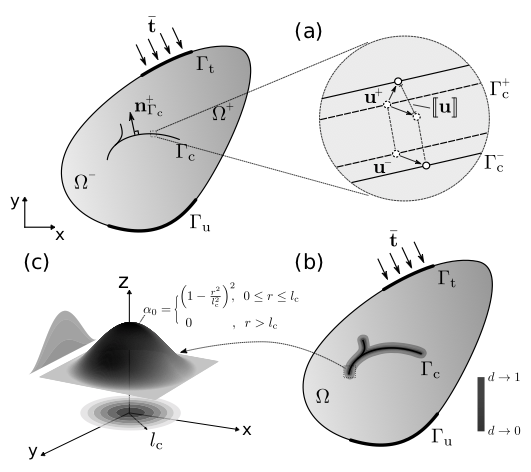
\includegraphics[width=5cm]{figures/Schematic_figure_LIE_PF_NLD}
\caption{Overview of the GeomInt Numerical Platform}
\label{fig:ogs-fem}
\end{wrapfigure}
